\documentclass[12pt,a4paper, xcolor=table]{article}
\usepackage{graphicx}
\usepackage[utf8]{inputenc}
\usepackage{eurosym}
\usepackage[spanish,es-tabla]{babel}
\usepackage[left=2cm, right=2cm, top=2cm, bottom=2cm]{geometry}
\usepackage{afterpage}
\PassOptionsToPackage{hyphens}{url}\usepackage{hyperref}
\usepackage{subfig}
\usepackage[table,xcdraw]{xcolor}


\usepackage{imakeidx}
\newcommand\blankpage{%
    \null
    \thispagestyle{empty}%
    \addtocounter{page}{-1}%
    \newpage}
\renewcommand*\contentsname{Índice: }

\makeindex
\let\olditemize\itemize
\def\itemize{\olditemize\itemsep=0pt}

\begin{document}
\setlength{\parindent}{0pt}
\begin{titlepage}
        \centering
        
\includegraphics[width=0.75\textwidth]{img/logo_uc3m.jpg}\par\vspace{3cm}
        {\huge\bfseries Práctica 1 \\ Aplicación de RNA\par}
        \vspace{0.5cm}
        {\scshape\Large Inteligencia Artificial en las Organizaciones\par}
        \vspace{1.5cm}
        {\scshape\Large Grupo 83-1\par}
        \vspace{1.5cm}
        {\Large\itshape Miguel Gutiérrez Pérez\par}
        {\Large 100383537@alumnos.uc3m.es \par}
        \vspace{1cm}
        {\Large\itshape Mario Lozano Cortés\par}
        {\Large 100383511@alumnos.uc3m.es\par}
        \vspace{1cm}
        {\Large\itshape Alba Reinders Sánchez\par}
        {\Large 100383444@alumnos.uc3m.es\par}
        \vspace{1cm}
        {\Large\itshape Alejandro Valverde Mahou\par}
        {\Large 100383383@alumnos.uc3m.es\par}
        \vfill

% Bottom of the page
        {\large \today\par}
\end{titlepage}

\tableofcontents

\newpage

\section{Introducción}

    El objetivo de la asignatura de Inteligencia Artificial en las Organizaciones es poner en relieve el encaje de las diversas técnicas de IA en contextos reales. Con esta motivación en mente, parece evidente que es imprescindible lograr obtener soluciones a problemas apremiantes con el conjunto de técnicas disponibles. Por su parte, la \textbf{epidemia} del\textbf{ SARS-CoV-2 }supone un \textbf{reto} para la humanidad, y constituye una oportunidad para demostrar el potencial de las nuevas herramientas de IA de las que disponemos para hacer frente a este nuevo desafío.

  \vspace{3mm}

  Uno de los \textbf{modelos computacionales} cuya aplicación resulta atractiva es el de las \textbf{Redes de Neuronas Artificiales}. La capacidad de aprender de grandes conjuntos de datos hacen de esta una opción perfecta para comprender y predecir los contagios causados por el virus.

  \vspace{2mm}

  Para comprender cómo cumplir con este objetivo debemos tener en cuenta cómo es posible que una red de neuronas aprenda. La respuesta se haya en su estructura. A nivel básico la estructura de una RNA supone un conjunto de entradas multiplicadas por unos pesos a modo de impulso nervioso al que se le puede aplicar determinadas funciones de activación. Dicha estructura de una neurona puede ser vista a continuación.

  \begin{figure}[h]
      \centering
      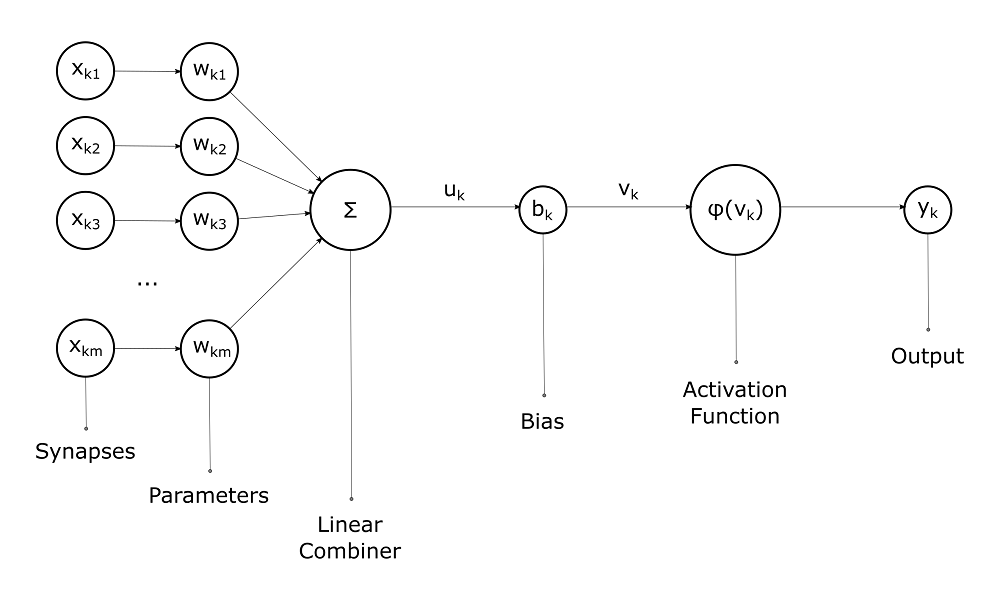
\includegraphics[width=400px]{img/Neuron.png}
      \captionsetup{labelformat=empty}
      \caption{Estructura de una neurona}
      % \label{fig:graf_exp1}
  \end{figure}

  Por lo tanto, hemos trasladado el problema a la \textbf{selección de los pesos} precisos para realizar predicciones lo más exactas posibles. El modelo a emplear se tratará del \textbf{Perceptrón Multicapa}. Consecuentemente el trabajo realizado en esta práctica consiste en \textit{tratar los datos para la aplicación del modelo elegido}, \textit{realizar los experimentos oportunos para dar con una configuración de la red apropiada} y \textit{analizar los resultados} obtenidos haciendo una reflexión crítica del proceso seguido.

  \vspace{5mm}

   La práctica se divide en dos partes: la primera trata de resolver un problema de \textbf{regresión} utilizando el \textbf{Perceptrón Multicapa}, y la segunda, de realizar predecicciones utilizando \textbf{series temporales} con la herramienta \textit{Weka}, y de nuevo, el \textbf{Perceptrón Multicapa}.

\newpage


\section{Parte 1: Regresión}

    \subsection{Planteamiento y desarrollo del problema a tratar}

    En esta primera parte se pretende predecir la transmisión del virus \textit{COVID-19} partiendo de un conjunto de datos que se explicarán en la siguiente sección. Se trata pues de un problema de regresión que se va a llevar a cabo mediante una RNA, a la que se van a modificar sus parámetros hasta conseguir aquellos con los que se genere un modelo con menor error a la hora de predecir.

    \vspace{2mm}

    El objetivo es predecir con la mayor exactitud posible los valores en 1, 2 y 3 días a futuro en dos países: \textbf{España} y \textbf{Brasil}. Para ello, se entrena una red con todos los datos, y se aplica la predicción sobre estos dos.

    \vspace{2mm}

    Para realizar la predicción en 2 y 3 días a futuro, se toman como entrada, además de los valores reales, los valores que la red ha predicho anteriormente.




    \subsection{Tratamiento de datos}

    Los datos que se han utilizado pertenecen al \textit{Novel Coronavirus (COVID-19) Cases Data} de la página \textit{The Humanitarian Data Exchange}[Referencia 4], se trata de una recopilación de \textbf{datos epidemiológicos del COVID-19} desde el día 22 de enero de 2020.

    \vspace{3mm}

    En concreto, los datos de interés son los que se encuentran en el fichero de casos diarios confirmados, este está compuesto de \textbf{266} provincias/estados de distintos países/regiones, de los cuales se recopila el \textbf{número de infectados totales} desde el 22 de enero hasta la fecha.

    \vspace{1mm}

    Los primeros atributos son: nombre de la provincia/estado, país/región, longitud y latitud (del país). Seguidos del número de contagiados acumulados por día.

    \vspace{3mm}

    El tratamiento de los datos que se ha llevado a cabo es el siguiente:

    \begin{itemize}
        \item En primer lugar, se ha eliminado la comilla simple del nombre de un país del fichero.
        \item Se han renombrado los atributos correspondientes a las fechas de forma que el día actual se convierte en \textit{Día 0} y el resto en \textit{Día -1}, \textit{Día -2},\dots
    \end{itemize}




    \subsection{Acercamiento con WEKA}

      Para poder trabajar con la herramienta \textit{WEKA} se transforma el fichero de formato \textit{.csv} a \textit{.arff}. Como la configuración por defecto que ofrece \textit{WEKA} para el algoritmo del perceptrón multicapa no es adecuada para la resolución del problema, es necesario alterar sus parámetros. Los valores que admiten modificación son:

      \begin{itemize}
        \item Número de ciclos
        \item Tasa de aprendizje
        \item Número de capas ocultas
      \end{itemize}

      Para poder realizar varios experimentos con distintos modelos y configuraciones diferentes, se usa la herramienta \textit{Experimenter} de \textit{WEKA}.

      \vspace{1mm}

      Debido a la cantidad de tiempo requerido para realizar el entrenamiento y a distintos problemas como: errores al leer los datos, valores de error extremadamente altos en algunos experimentos, poca precisión de los modelos y falta de personalización de la red, se decide descartar este acercamiento por uno que permite resolver estos problemas de manera sencilla.




    \subsection{Acercamiento con Python-Tensorflow}

    La principal ventaja de la biblioteca \textit{Tensorflow} es la personalización de las redes. Esto permite la modificación de valores como la función de coste, la función de optimización, o el número de neuronas por cada capa de la red. Además, junto a la biblioteca de cálculo numérico \textit{numpy} permite que el entrenamiento de estas redes sea mucho más ágil.

    \vspace{3mm}

    Una de las facilidades que ofrece es la capacidad de crear redes neuronales de forma rápida, y poder entrenarla y realizar predicciones con apenas unas líneas de código.

    \vspace{2mm}

    Gracias a esta tecnología ha sido posible realizar distintos experimentos hasta que se ha encontrado la configuración de la red que es capaz de resolver el problema de la mejor manera.

    \vspace{3mm}

    Para realizar la lectura de los datos se ha hecho uso de la biblioteca \textit{pandas}, concretamente, la función de \textit{read\_csv}. Después, se ha transformado en una lista de \textit{numpy}, lo que ha facilitado su manejo dividiendo los datos e forma rápida y sencilla.

    \vspace{4mm}

    Se han creado 3 archivos de \textit{Python} con el propósito de resolver el problema:

    \begin{enumerate}
      \item \textbf{Perceptrón con 'K Fold'}[Anexo 1]

        Este primer archivo usa una función de la bibioteca \textit{sklearn} que implementa el algoritmo '\textit{K Fold}'. Se ha decidido realizar la división de los datos en 10 partes.

        \vspace{2mm}

        El archivo genera y guarda los modelos para, posteriormente, poder usarlos en la predicción.

      \item \textbf{Perceptrón con 'split percentage'}[Anexo 2]

        El segundo archivo genera modelos entrenados usando la técnica de división de datos en conjunto de entrenamiento y de test. Estos modelos también se guardan para poder realizar predicciones con los mismos.

      \item \textbf{Predicción usando los modelos generados}[Anexo 3]

        El archivo realiza la predicción, usando los modelos cargados, con los dos países seleccionados (España y Brasil). Las predicciones se realizan, como se ha explicado antes, sobre el primer día usando los datos reales. Después, los datos reales, junto a este primer día predicho, se usan para realizar la predicción del segundo día. El mismo proceso se hace para realizar la tercera predicción.

    \end{enumerate}




    \subsection{Configuración de experimentos con MLP}

      Se han planteado 4 modelos en función de los días seleccionados para entrenar a la red: modelo con 7 días, modelo con 15 días, modelo con 30 días y modelo con 60 días.

      \vspace{2mm}

      Se ha elegido esta división, que corresponden con 1 semana, 2 semanas, 1 mes y 2 meses respectivamente, ya que se quiere comprobar cuánto tiempo es necesario conocer de antemano para preever la evolución de infectados por \textit{COVID-19} en una región.

      \vspace{2mm}

      Se han realizado distintos experimentos con cada modelo, dividiendo entre el algoritmo de '\textit{K Fold}' y '\textit{percentage split}' para encontrar aquel que genere los mejores resultados.

      \vspace{3mm}

      Los hiperparámetros comunes a todos los modelos son:

      \begin{itemize}
        \item \textbf{Número de capas ocultas}: son aquellas capas de una red neuronal que no son ni de entrada ni de salida. No se ha utilizado \textbf{ninguna} capa oculta, porque los resultados experimentales proporcionan mayor precisión si no se usan. Además, tanto la herramienta de \textit{WEKA} como los modelos generados con \textit{Tensorflow} coincidían en esta arquitectura.
        \item \textbf{Tasa de aprendizaje}: es el factor por el que se multiplica el gradiente durante el entrenamiento de la red, generando el paso de gradiente, utilizado para actualizar los pesos. Se ha usado el valor que ofrece la biblioteca \textit{Tensorflow} por defecto en el optimizador, \textbf{0.001}.
        \item \textbf{Número de ciclos}: es el número de veces que la red realiza el bucle de entrenamiento sobre todos los datos. Se han utilizado \textbf{500} ciclos porque a partir de este valor las mejoras de los modelos no eran significativas.
        \item \textbf{Optimizador}: es la función encargada de encontrar el mínimo local de la función de coste y actualizar los pesos de la red en consecuencia. En este caso el elegido es \textbf{Adam} ya que es una versión del descenso del gradiente que genera mejores resultados.
        \item \textbf{Función de coste}: es la función que indica el error de la red. En este caso se ha usado el \textbf{error medio absoluto}, dado que se trata de un problema de regresión. Otra posible opción habría sido el error cuadrático medio.
        \item \textbf{Función de activación}: es la función de cada neurona que toma como entrada la suma de todas las salidas de la capa anterior y genera una salida no lineal para la siguiente capa. En los modelos se usa la función \textbf{ReLU} en las capas ocultas, y la función \textbf{linear} en las capas de salida, ya que se trata de un problema de regresión.

      \end{itemize}


      Los parámetros que se modifican entre los modelos son el algoritmo usado para generar el modelo, el número de entradas de la red, y el número de neuronas en la capa de entrada.

      \begin{table}[h]
        \centering
      \begin{tabular}{|c|c|c|c|}
      \hline
      \rowcolor[HTML]{FFCE93}
      \textbf{Algoritmo} & \textbf{Entradas red} & \textbf{Neuronas capa entrada} & \textbf{Error mejor experimento} \\ \hline
      K Fold             & 7                     & 64                             & 4076.555                         \\ \hline
      Split              & 7                     & 64                             & 1378.325                         \\ \hline
      K Fold             & 15                    & 64                             & 2138.145                         \\ \hline
      Split              & 15                    & 64                             & 2141.331                         \\ \hline
      K Fold             & 30                    & 128                            & 2942.597                         \\ \hline
      Split              & 30                    & 128                            & 10260.810                        \\ \hline
      K Fold             & 60                    & 128                            & 3031.660                         \\ \hline
      Split              & 60                    & 128                            & 8037.908                         \\ \hline
    \end{tabular}
      \end{table}

    A pesar de que unos modelos puedan mostrar menor error, no tiene por qué ser ese modelo el mejor. Hasta que no se pruebe con casos reales no se podrá asegurar que uno es mejor que otro.

      \vspace{2mm}

    Aún así, según refleja la tabla, el error cometido con el algoritmo \textit{K Fold} es menor en todos los casos excepto en el que sólo hay 7 entradas en la red.




    \subsection{Análisis de resultados}

    En primer lugar se van a analizar los resultados obtenidos acerca de la predicción de los contagiados en \textbf{España}, usando gráficas que permitan comparar los distintos modelos generados, en función a sus resultados y sus errores, y a continuación, se realizará el mismo proceso con los datos de \textbf{Brasil}.

    \subsubsection{Resultados de España}

    Las siguientes dos gráficas muestran las predicciones de los modelos respecto a los datos de España. Se ha decidido mostrar hasta 11 días atrás para poder observar la evolución de los datos con perspectiva.

    \begin{center}
        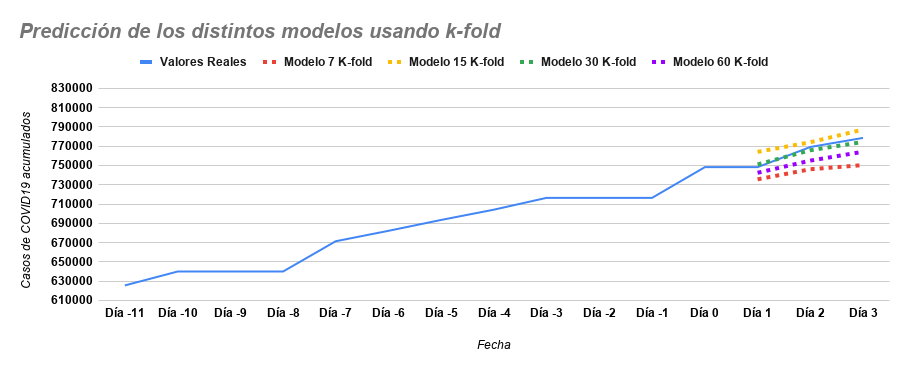
\includegraphics[width=450px]{img/pred_modelos_kFold_ES.png}
    \end{center}

    \begin{center}
        \centering
        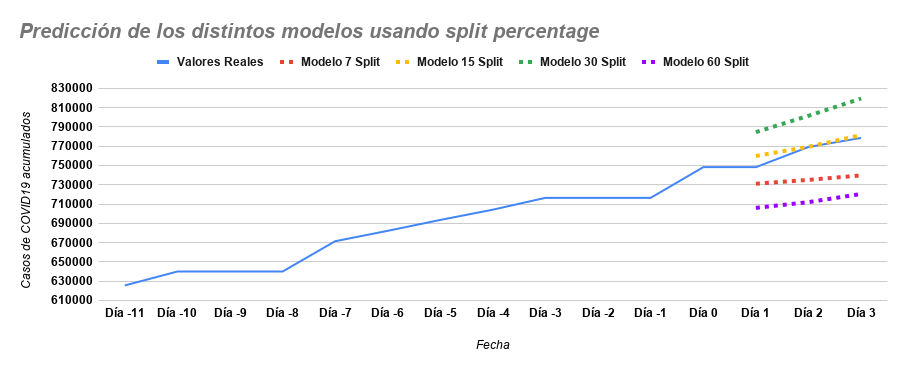
\includegraphics[width=450px]{img/pred_modelos_split_ES.png}
    \end{center}

    Se puede observar gráficamente que los mejores modelos para este problema son el \textbf{Modelo 30 K Fold} y el \textbf{Modelo 15 Split}. A pesar de esto, los modelos de \textit{K fold} se acercan mucho más a los valores reales, y se puede atribuir la precisión del \textbf{Modelo 15 Split} al azar.

    \vspace{3mm}

    La siguiente gráfica muestra la evolución del error absoluto en función de los días predichos.

    \begin{center}
        \centering
        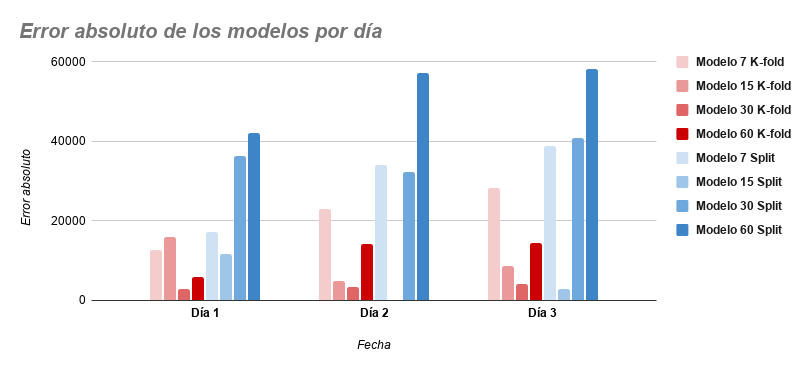
\includegraphics[width=450px]{img/error_modelos_ES.png}
    \end{center}

    Esta gráfica demuestra que la previsión acertada del \textbf{Modelo 15 Split} es fruto del azar, porque en el primer día muestra un gran error, que corrige en el segundo día, y se vuelve a incrementar en el tercero. Si realmente fuera capaz de realizar previsiones acertadas, el error debería ser incremental a lo largo del tiempo.

    \vspace{2mm}

    Viendo los resultados de las dos gráficas, junto a la gráfica de error, se considera por tanto que los modelos que usan \textbf{K Fold} son mejores para este problema, concretamente, el mejor para el caso de España es el \textbf{K Fold con datos de 30 días}.



    \subsubsection{Resultados de Brasil}

    En el caso de Brasil se muestran, al igual que en el caso de España, hasta 11 días atrás, ya que se observa mejor la evolución de los datos.

    \begin{center}
        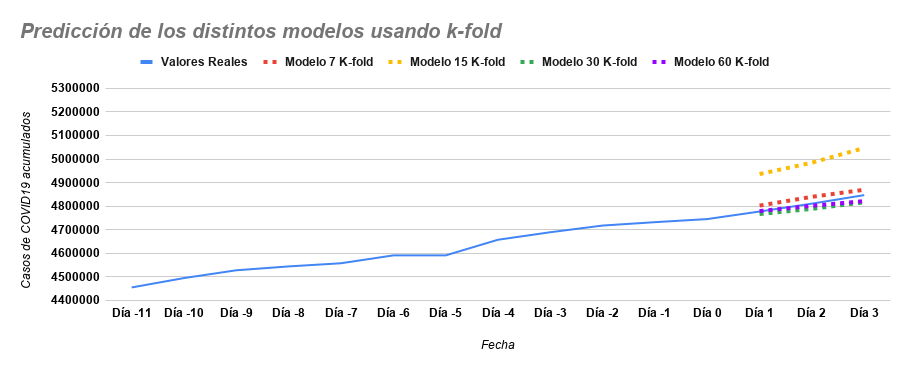
\includegraphics[width=450px]{img/pred_modelos_kFold_BZ.png}
    \end{center}

    \begin{center}
        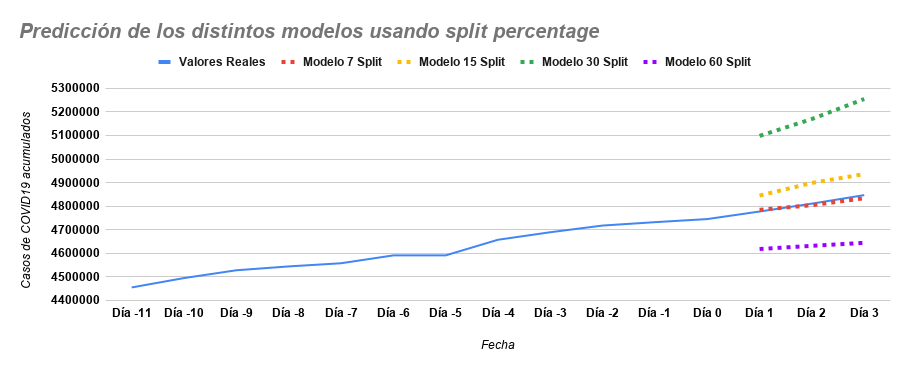
\includegraphics[width=450px]{img/pred_modelos_split_BZ.png}
    \end{center}

    Gráficamente, se observa que los mejores modelos para este problema son el \textbf{Modelo 60 K Fold}, el \textbf{Modelo 30 K Fold} y el \textbf{Modelo 7 Split}. Al igual que en el caso de España, los modelos de \textit{K fold} se acercan mucho más a los valores reales, y se puede atribuir la precisión del \textbf{Modelo 7 Split} al azar.

    \vspace{2mm}

    Esto se puede demostrar a su vez porque el \textbf{Modelo 7 Split} en el caso de España generaba resultados malos y el \textbf{Modelo 15 Split} que daba buenos resultados, en este caso no los da.

    \vspace{4mm}

    La siguiente gráfica muestra la evolución del error absoluto en función de los días predichos.

    \begin{center}
        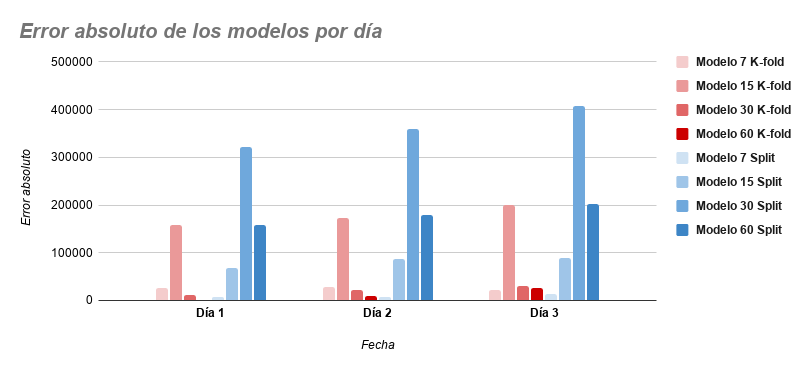
\includegraphics[width=450px]{img/error_modelos_BZ.png}
    \end{center}

    A pesar de que en esta gráfica el error de los modelos que usan \textit{split percentage} es proporcional según se aumenta el día a predecir, debido a los motivos discutidos en el apartado anterior (Resultados de España) y los motivos explicados en las gráficas anteriores, se ha decidido que para el caso de Brasil los mejores modelos sean el \textbf{Modelo 60 K Fold} y el \textbf{Modelo 30 K Fold}.

    \vspace{2mm}

    Dado que el \textbf{Modelo 30 K Fold} es el que mejores resultados produce como regla general, se considera que el mejor modelo para resolver el problema de predecir los contagiados de un país cualquiera es \textbf{K Fold con datos de 30 días}.

    \vspace{6mm}

    \textit{Para ver información más detallada de las gráficas y sus valores, consultar [Anexo 4]}.



    \newpage
    \section{Parte 2: Series temporales}

    \subsection{Descripción de las series temporales utilizadas}

        Se puede definir las series temporales como un una \textbf{sucesión de datos o muestras medidos en intervalos de tiempo regulares} de los cuales resulta especialmente interesante el factor de predicción de los valores en instantes de tiempo futuros. Dichas predicciones son posibles al detectar patrones o tendencias en los datos a lo largo del tiempo.

        \vspace{2mm}

        La pregunta que se debe hacer es si se corresponden los datos de contagios acumulados y muertes por territorios del  \textit{SARS-CoV-2} con una serie temporal de la que se puedan realizar predicciones fiables. Para contestar a esta pregunta hay que fijarse en las variables de las que se disponen y la relación entre ambas. Como variable independiente se cuenta con el tiempo, mientras que el número de contagios (o fallecidos, según el caso) se identifica con la variable dependiente, puesto que esta cifra depende en gran medida del la cifra medida en el instante de tiempo anterior. Por lo tanto \textbf{se trata de una serie temporal}.

        \vspace{2mm}

        Sin embargo, existen más características en las que uno se puede fijar. [Referencia 2]

    \begin{itemize}
    \item \textbf{Estacionalidad}: Se refiere a fluctuaciones periódicas. Un análisis en profundidad de los datos de la epidemia debería considerar este factor, no obstante, dado que la pandemia no lleva entre nosotros un periodo de tiempo lo suficientemente grande como para detectar un comportamiento estacional a lo largo de las distintas épocas del año no nos fijaremos en este parámetro.
    \item \textbf{Estacionaridad}: No debe ser confundido con la estacional dado que hace referencia al mantenimiento de los valores estáticos tales como la media y varianza. El proceso de crecimiento descontrolado de una pandemia no puede ser considerado estacionario debido a la tendencia alcista y volátil de los datos.
    \end{itemize}

    A continuación se muestra un ejemplo de una serie temporal estacional y estacionaria para comprobar cómo difiere de la serie temporal de los datos del \textit{COVID} mundiales.

        \begin{figure}[h]
                \centering
                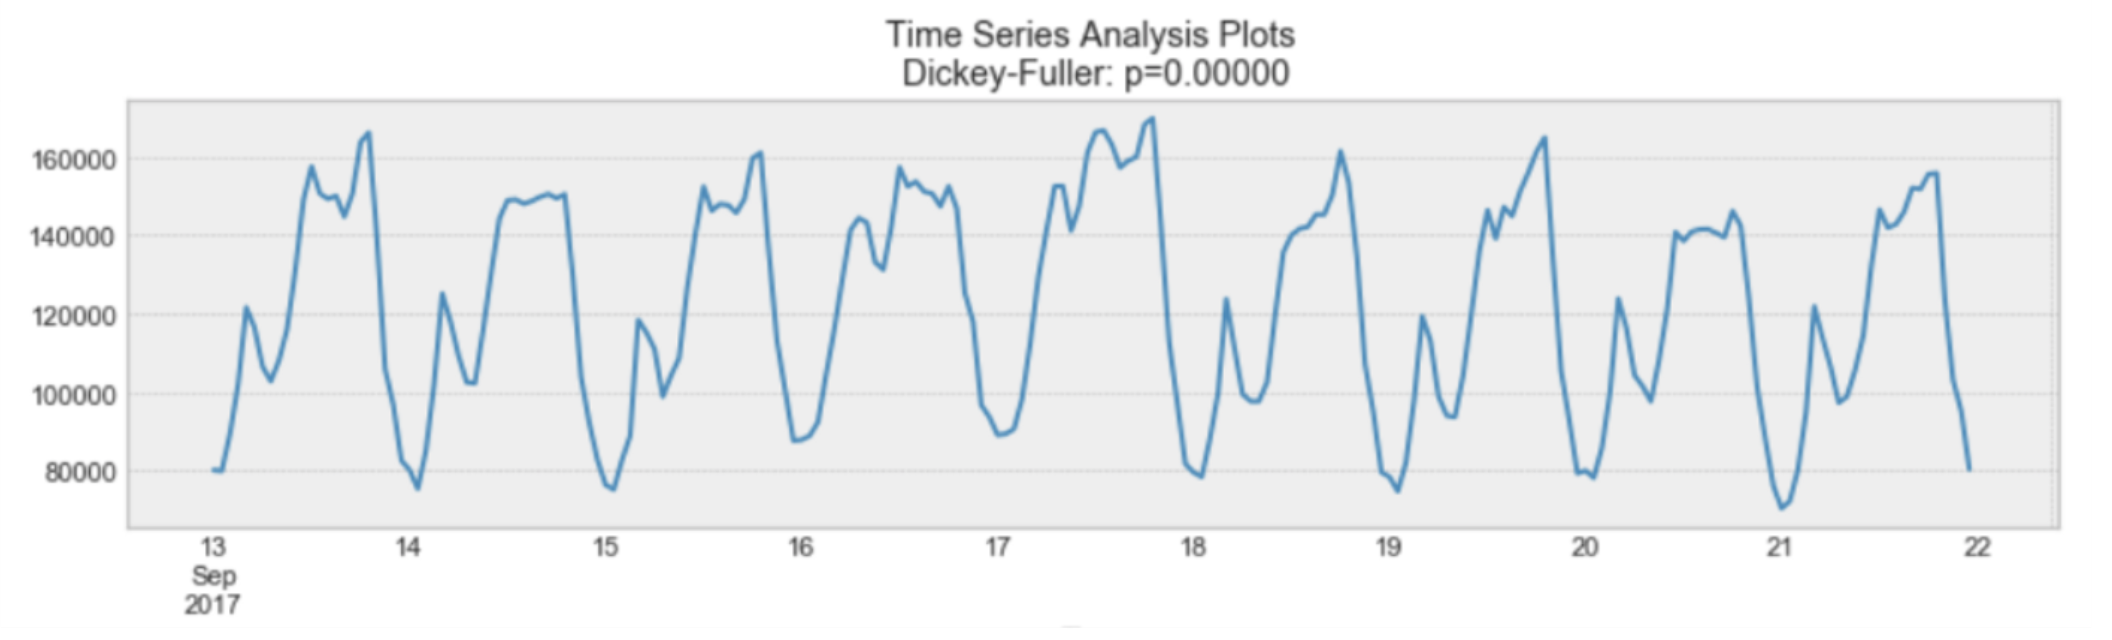
\includegraphics[width=320px]{img/estacional.png}
                \captionsetup{labelformat=empty}
                \caption{Serie temporal estacional y estacionaria}
                % \label{fig:graf_exp1}
            \end{figure}





        \begin{figure}[h]
                \centering
                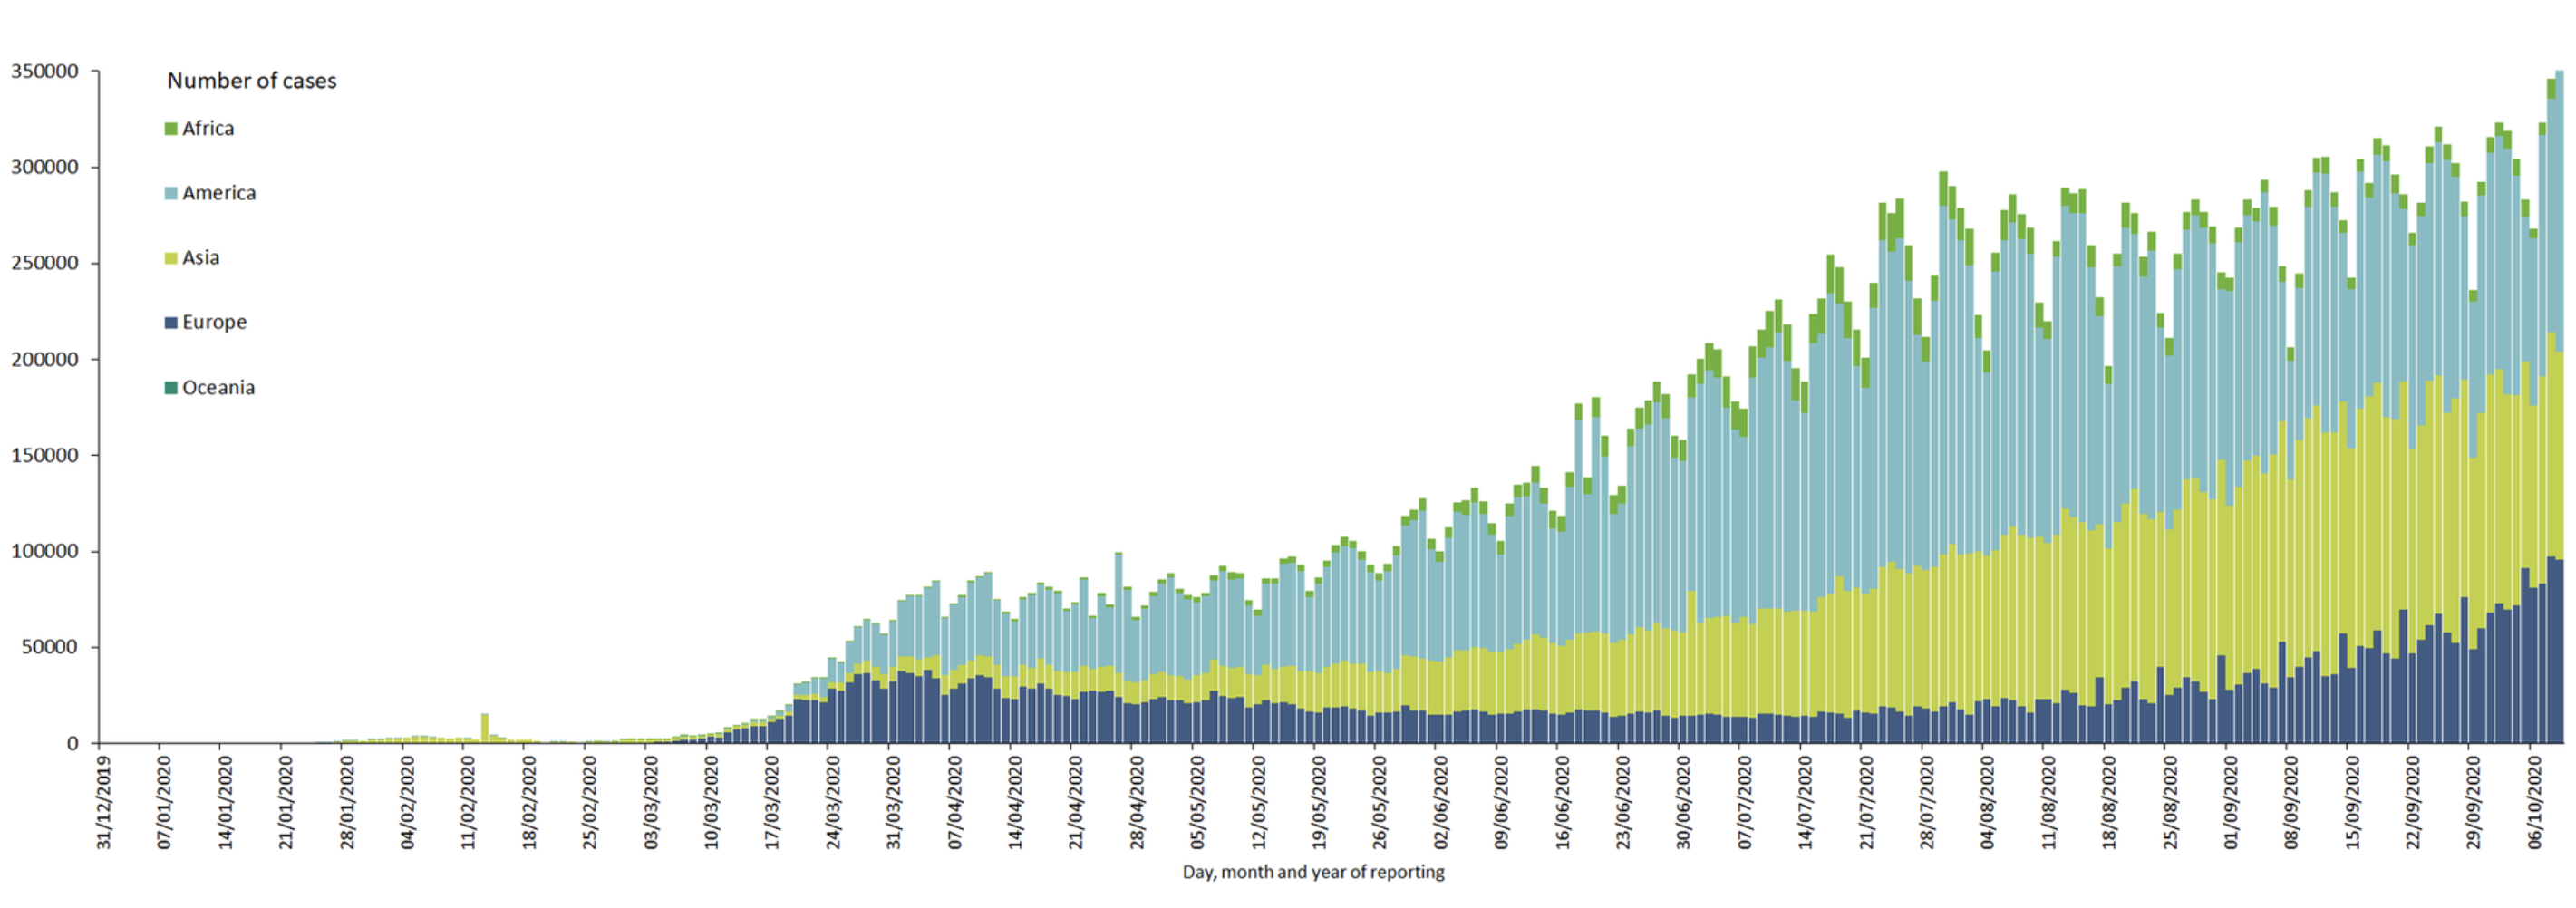
\includegraphics[width=320px]{img/covid-cases.png}
                \captionsetup{labelformat=empty}
                \caption{Casos mundiales de \textit{COVID}. [Referencia 3]}
                % \label{fig:graf_exp1}
            \end{figure}

    \subsection{Proceso de experimentación}
    La red de neuronas generada seguirá el algoritmo de \textit{Multilayer Perceptron }para la predicción de series temporales en el apartado \textit{timeseriesForecasting} de \textit{Weka}. Por lo tanto, el siguiente paso consiste en la selección de los parámetros de la red que permitan encontrar la mejor predicción posible.

        \subsubsection{Arquitecturas probadas}

        En el caso de \textit{Multilayer Perceptron } existen multitud de parámetros de los cuales debemos considerar su variación y combinación para obtener una buena arquitectura de red. Algunos de ellos (\textit{número de capas ocultas, tasa de aprendizaje y tiempo de entrenamiento}) han sido descritos en la la sección Parte 1 de esta memoria y por tanto se obvia la explicación. Sin embargo, la aproximación con series temporales introduce un nuevo parámetro a explicar. La definición del mismo se da a continuación.

        \begin{itemize}
        \item \textbf{Longitud de retraso (Lag Lenght)}: Las variables \textit{lag} son el mecanismo por el cual se determina la \textbf{relación entre las variables pasadas y las tratadas actualmente}. Una forma de pensar en este parámetro consiste en equipararlo a la longitud de la ventana de tiempo en la que se tiene en cuenta el valor de las variables pasadas. Por consiguiente, \textbf{un valor apropiado de este parámetro en el caso considerado es 7 días} dado que los estados suelen tener problemas en las notificaciones del fin de semana, siendo apropiado estudiar el efecto de la pandemia en porciones de una semana. Por lo tanto, se usarán 7 y 14 días para las pruebas.
        \end{itemize}

        Se concluye que es necesario realizar la siguiente aproximación a la arquitectura de la red mostrada en la tabla contigua, combinando adecuadamente valores lógicos de los parámetros propuestos.

        \begin{table}[h]
        \begin{tabular}{|c|c|c|c|c|}
        \hline
        \rowcolor[HTML]{DAE8FC}
        \textbf{ID} & \textbf{Longitud retraso} & \textbf{Cap ocultas} & \textbf{Tasa aprendizaje} & \textbf{Tiempo entrenamiento} \\ \hline
        1                       & 7                   & a                      & 0,1                    & 500                    \\ \hline
        2                       & 7                   & a                      & 0,1                    & 5000                   \\ \hline
        3                       & 7                   & a                      & 0,3                    & 500                    \\ \hline
        4                       & 7                   & a                      & 0,3                    & 5000                   \\ \hline
        5                       & 7                   & t                      & 0,3                    & 500                    \\ \hline
        6                       & 7                   & t                      & 0,3                    & 5000                   \\ \hline
        7                       & 7                   & t                      & 0,1                    & 500                    \\ \hline
        8                       & 7                   & t                      & 0,1                    & 5000                   \\ \hline
        9                       & 14                  & a                      & 0,1                    & 500                    \\ \hline
        10                      & 14                  & a                      & 0,1                    & 5000                   \\ \hline
        11                      & 14                  & a                      & 0,3                    & 500                    \\ \hline
        12                      & 14                  & a                      & 0,3                    & 5000                   \\ \hline
        13                      & 14                  & t                      & 0,3                    & 500                    \\ \hline
        14                      & 14                  & t                      & 0,3                    & 5000                   \\ \hline
        15                      & 14                  & t                      & 0,1                    & 500                    \\ \hline
        16                      & 14                  & t                      & 0,1                    & 5000                   \\ \hline
        \end{tabular}
        \end{table}

        Finalmente, es interesante destacar que cada uno de los experimentos debe ser dividido a su vez en \textit{4 sub-experimentos} debido a que la herramienta de \textit{forecasting} permite tomar los datos de contagios y muertes de manera aislada o de manera cruzada. Es decir, para cada una de las configuraciones de los experimentos debemos realizar uno con los datos de confirmados acumulados aislados, uno con los datos de los muertos aislados y otros dos con las series cruzadas. Los resultados de los experimentos se tratan en el siguiente apartado.

        \subsection{Análisis de resultados}
            El análisis de los resultados se realizará por separado para cada país. Tal y como se pedía, los diferentes modelos \textbf{han precedido 15 días} de diferentes series: confirmados aislados, fallecidos aislados, confirmados cruzados y fallecidos cruzados. Al disponer de los datos reales para esos días será posible medir el error, para el cual se usará el error medio absoluto de los 15 días, y para medir el error general, el error medio absoluto de las cuatro predicciones. Se empieza mostrando los resultados de todos los modelos para cada predicción, y finalmente se verá el error que cada modelo ha tenido de media. De esta manera, se descubre que modelo ha funcionado mejor con cada predicción y cual ha predecido bien de manera regular. Por último, dada la gran cantidad de modelos, se refiere a ellos según los identificadores que se encuentran en la tabla anterior.

            \subsubsection{Resultados de España}

            \begin{center}
                \centering
                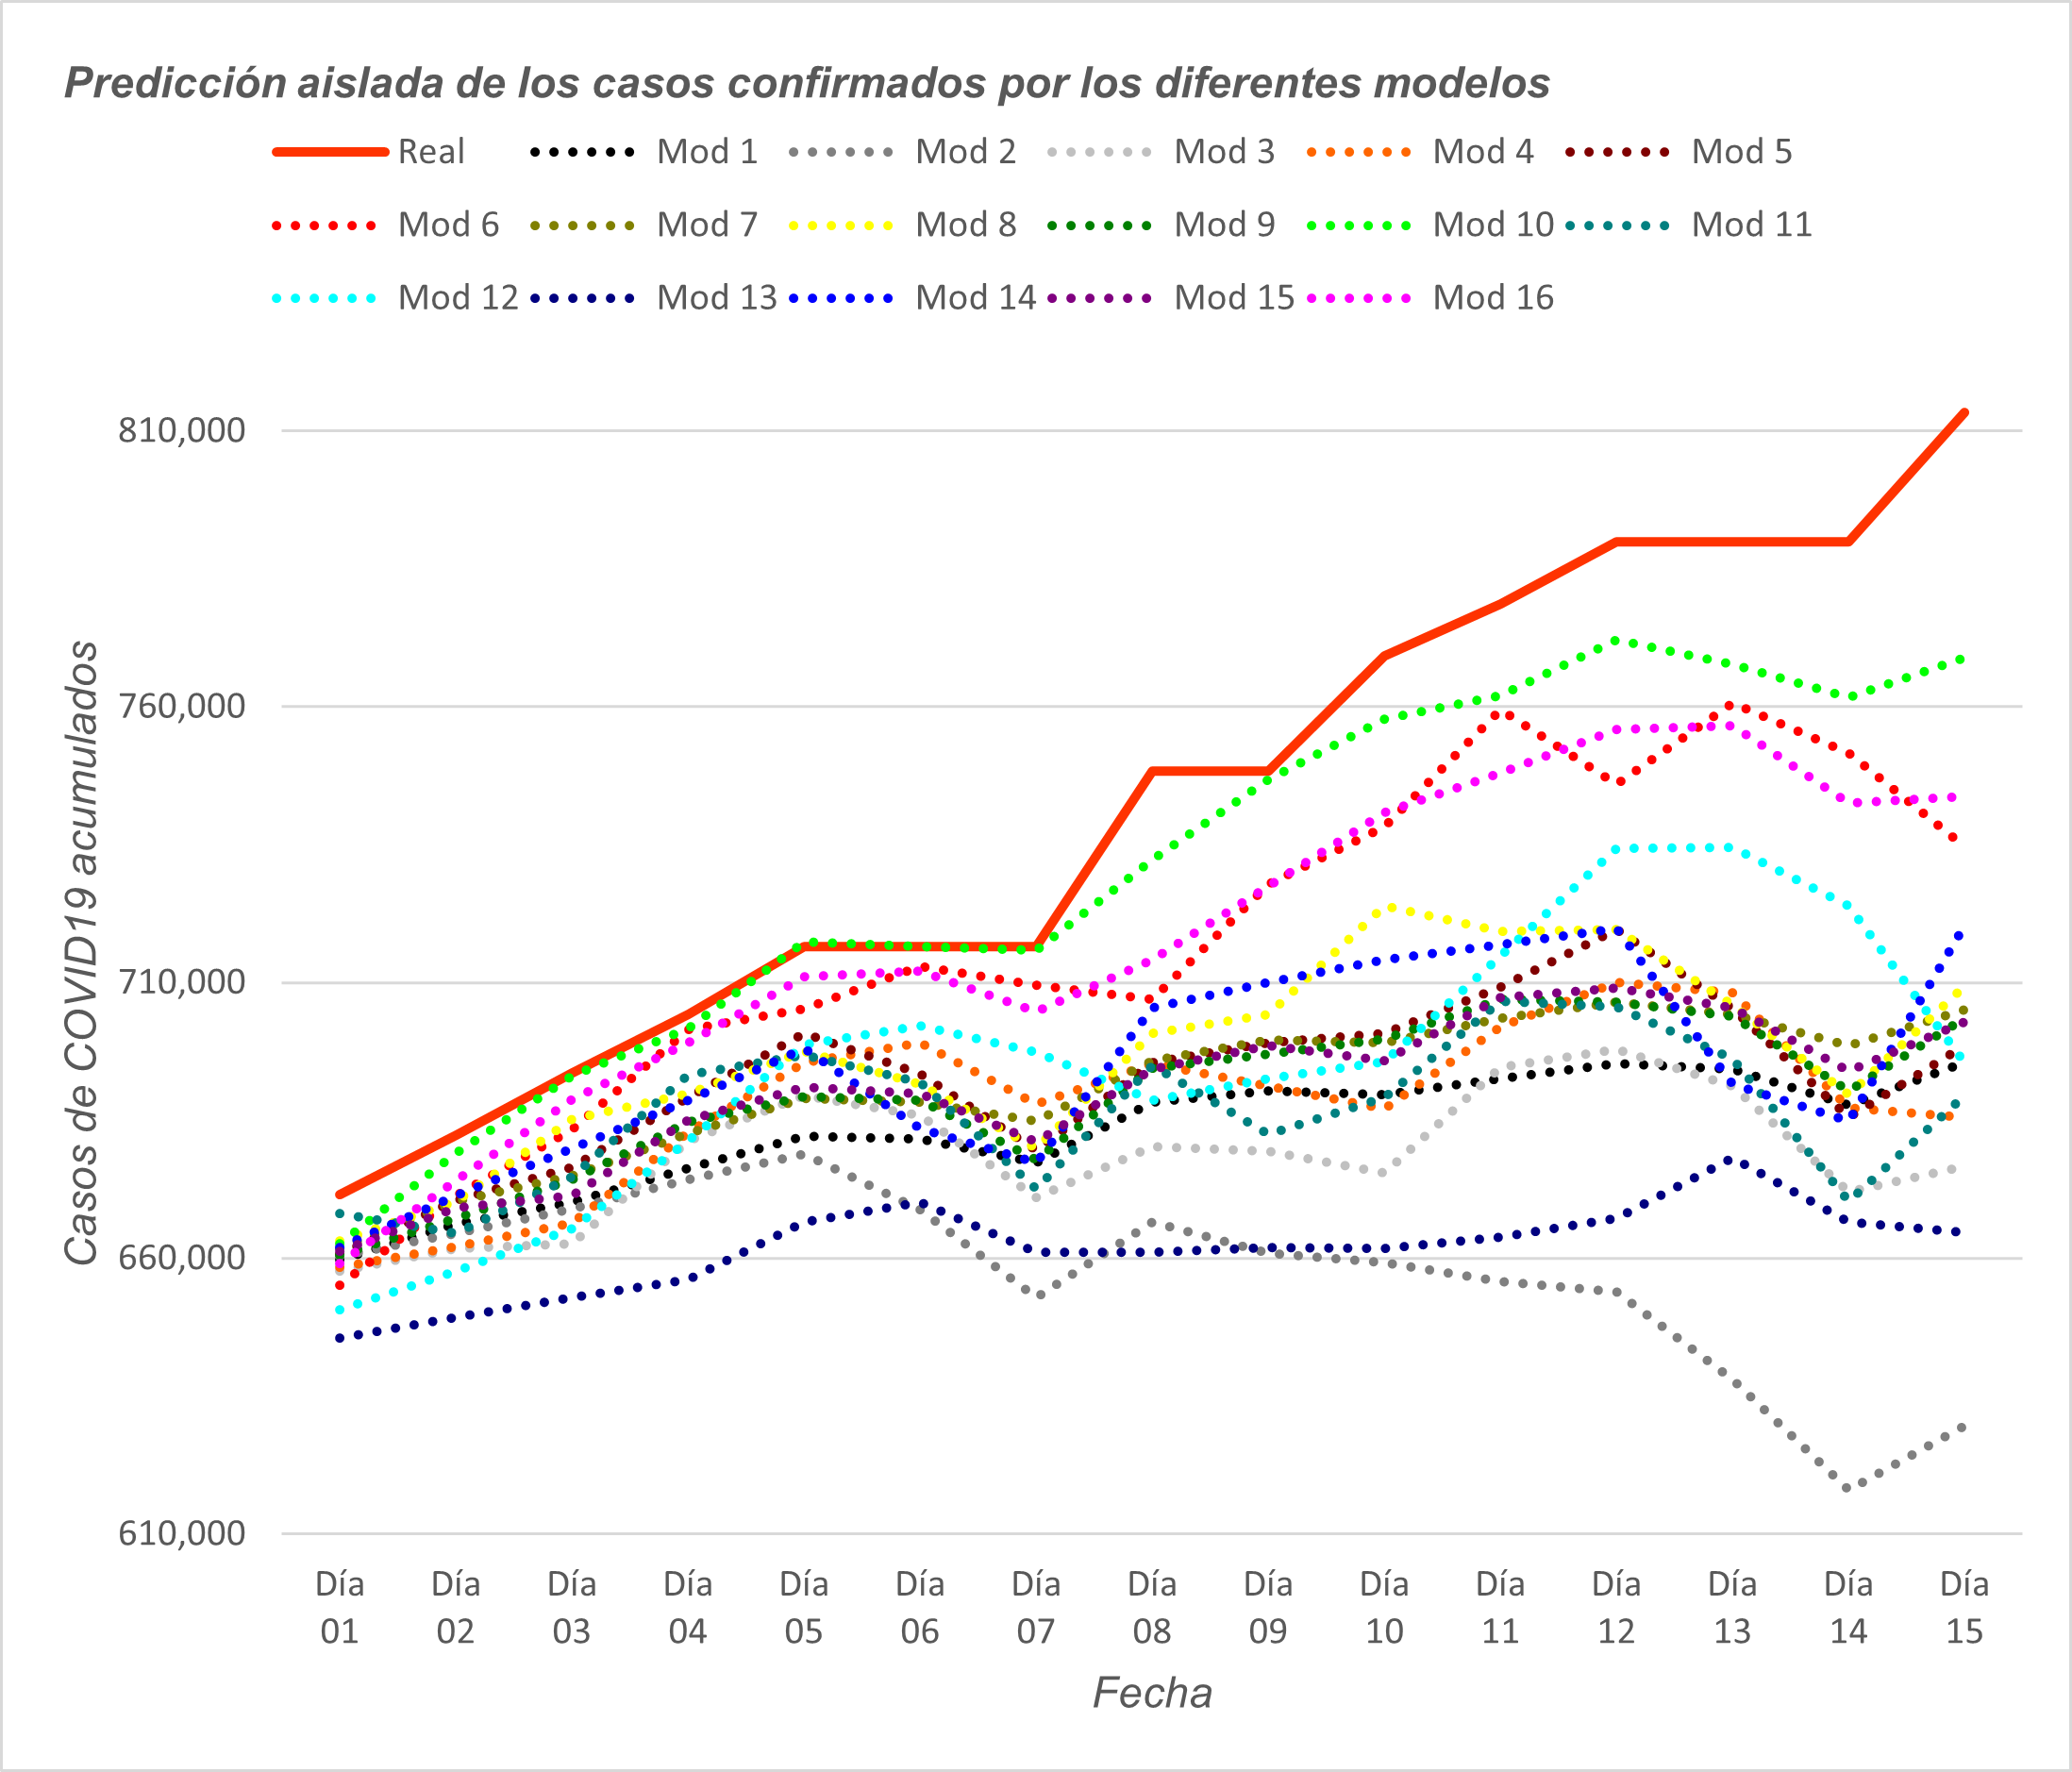
\includegraphics[width=450px]{img/pred_a_conf_ES.png}
            \end{center}

            En la primera imagen, correspondiente a la \textbf{predicción aislada de casos confirmados}, se ve como a simple vista los modelos no generan demasiado bien. \textbf{El que más se acerca es el modelo 10}. Sin embargo, todos los modelos presentan caídas y subidas de manera continuada, lo que es completamente erróneo, dado que los datos son acumulados.

            \begin{center}
                \centering
                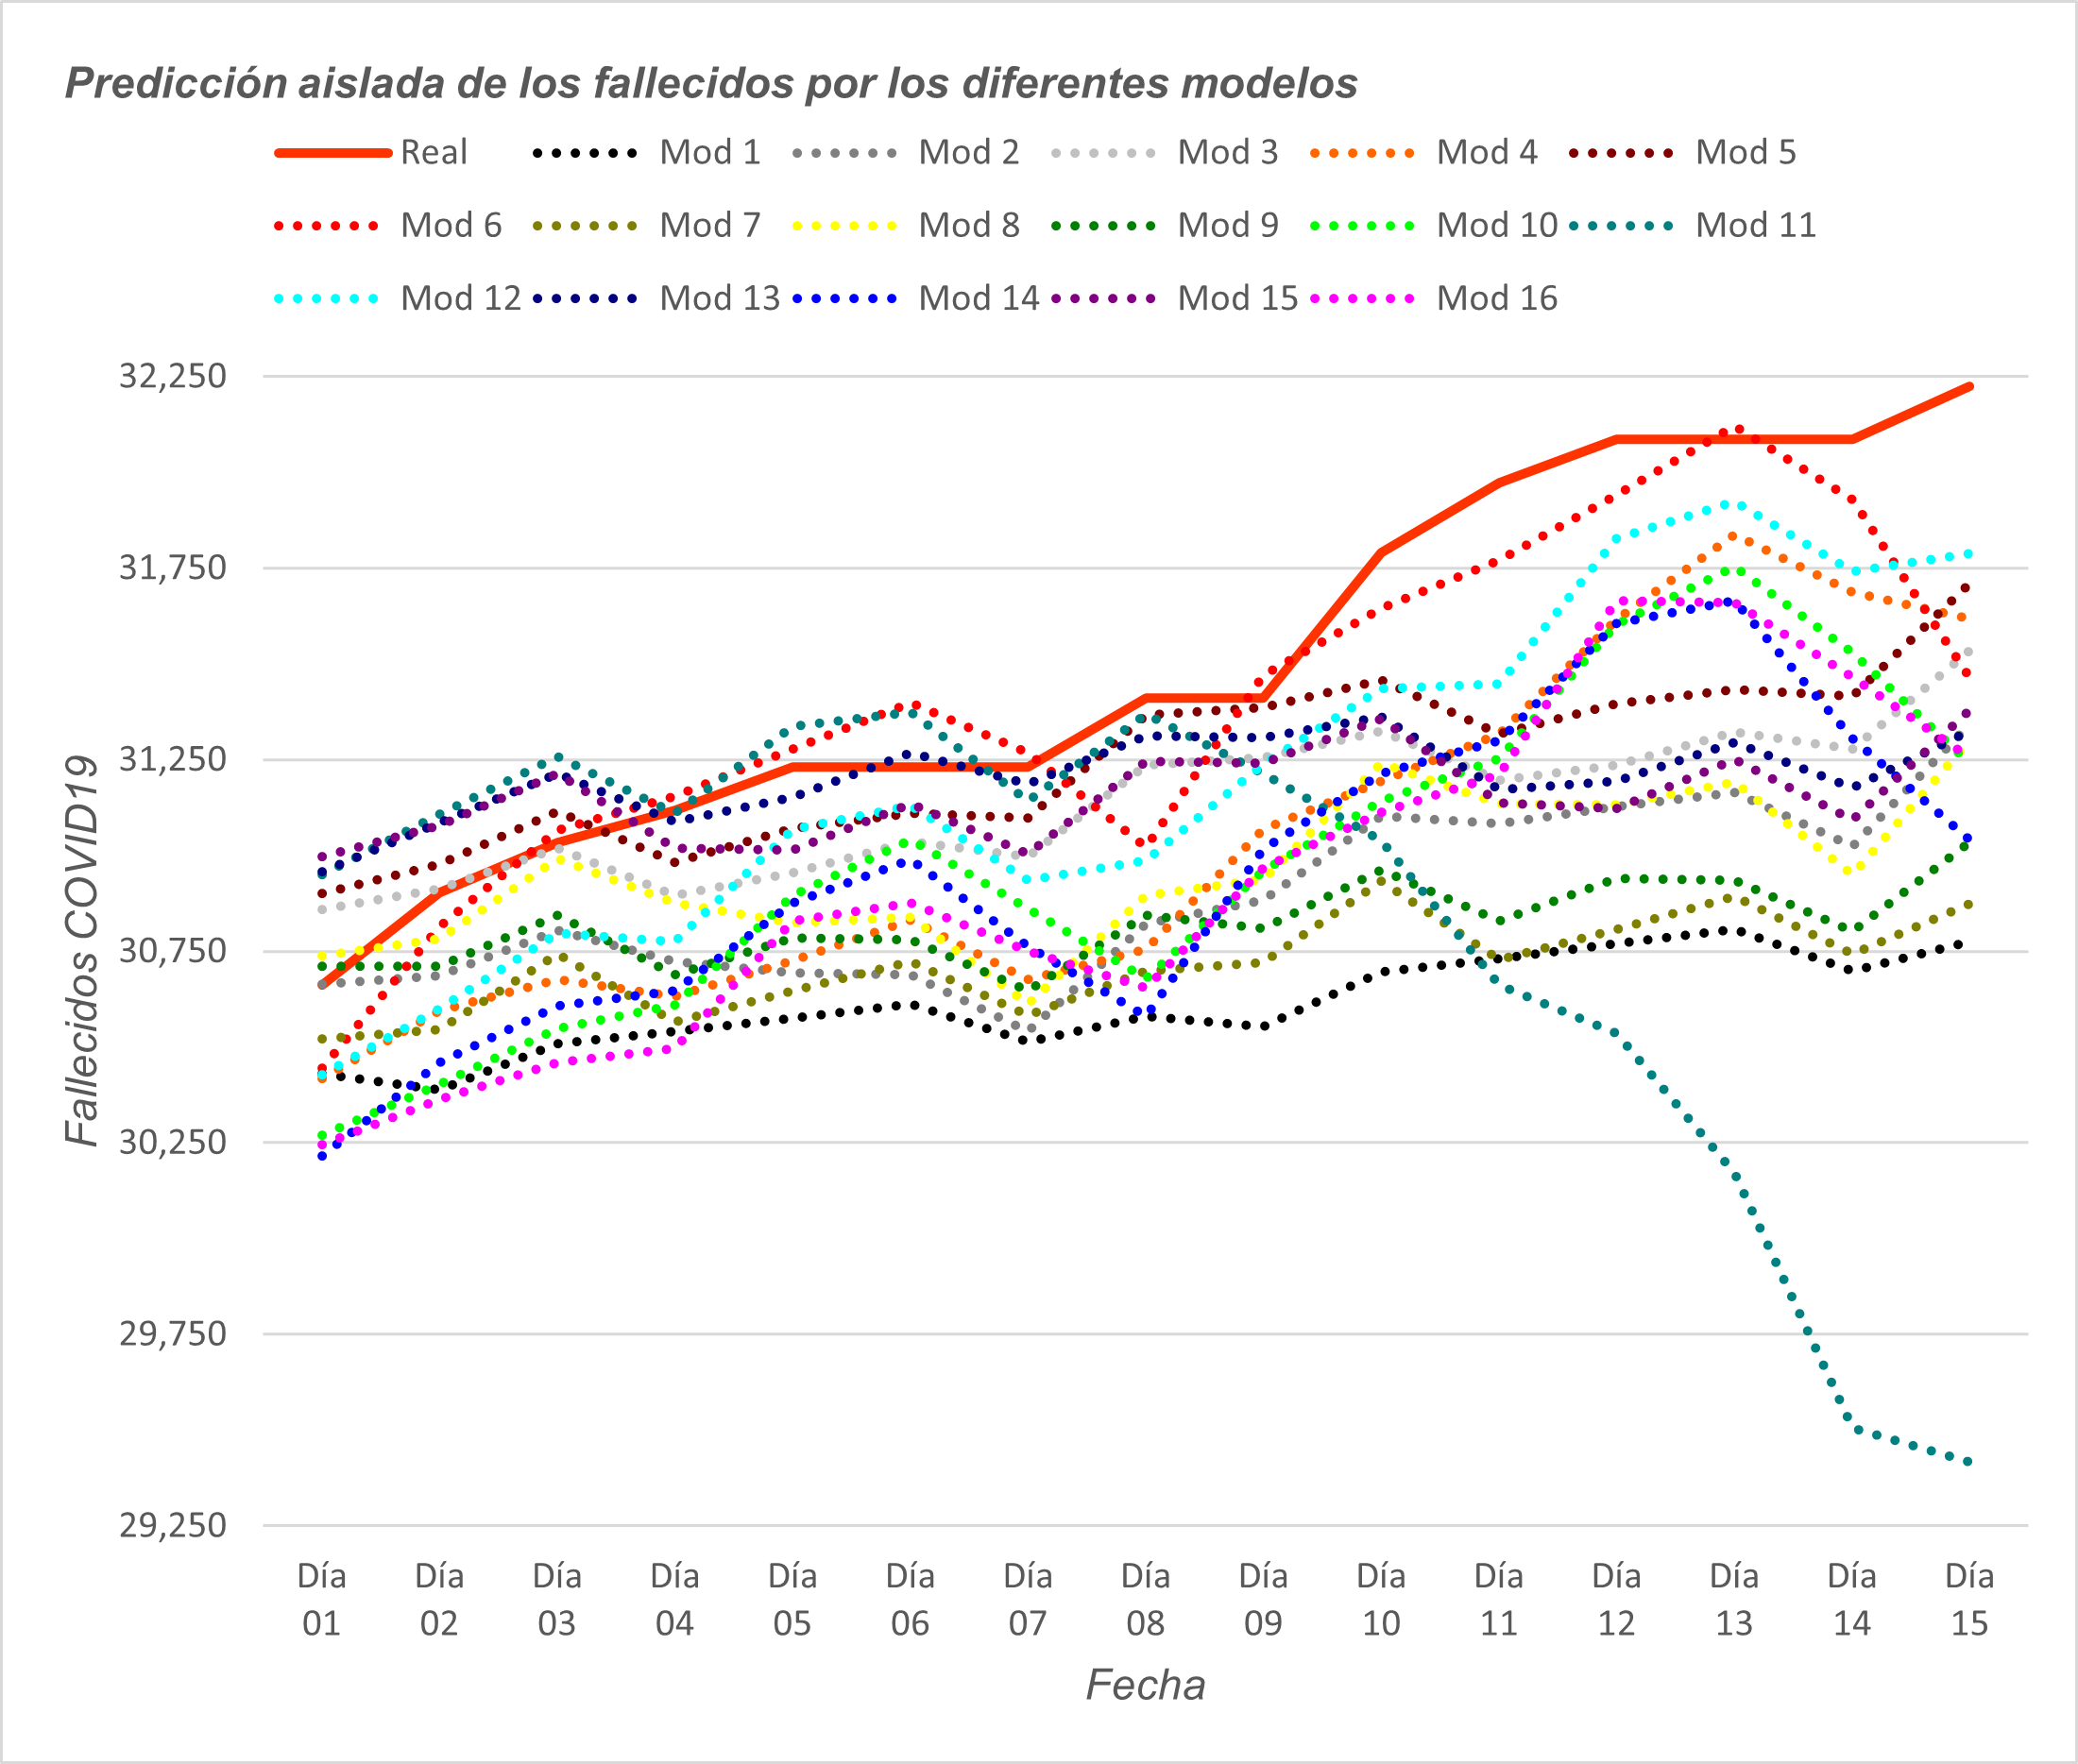
\includegraphics[width=450px]{img/pred_a_fall_ES.png}
            \end{center}

            A continuación, si tienen los datos de la \textbf{predicción aislada de fallecidos}. En esta ocasión, aunque tampoco son muy buenos, no son del todo malos, ya que el rango de valores en el que se mueven los modelos es bastante más pequeño, aunque tratándose de muertes, un número pequeño puede tener más importancia en la realidad. En este caso, \textbf{el modelo que parece acercarse más a los valores reales es el modelo 6}. Una cosa curiosa que pasa en esta predicción es el modelo 11, cuya predicción no hace más que decrecer, cosa de nuevo, totalmente errónea y sin ningún sentido.

            \begin{center}
                \centering
                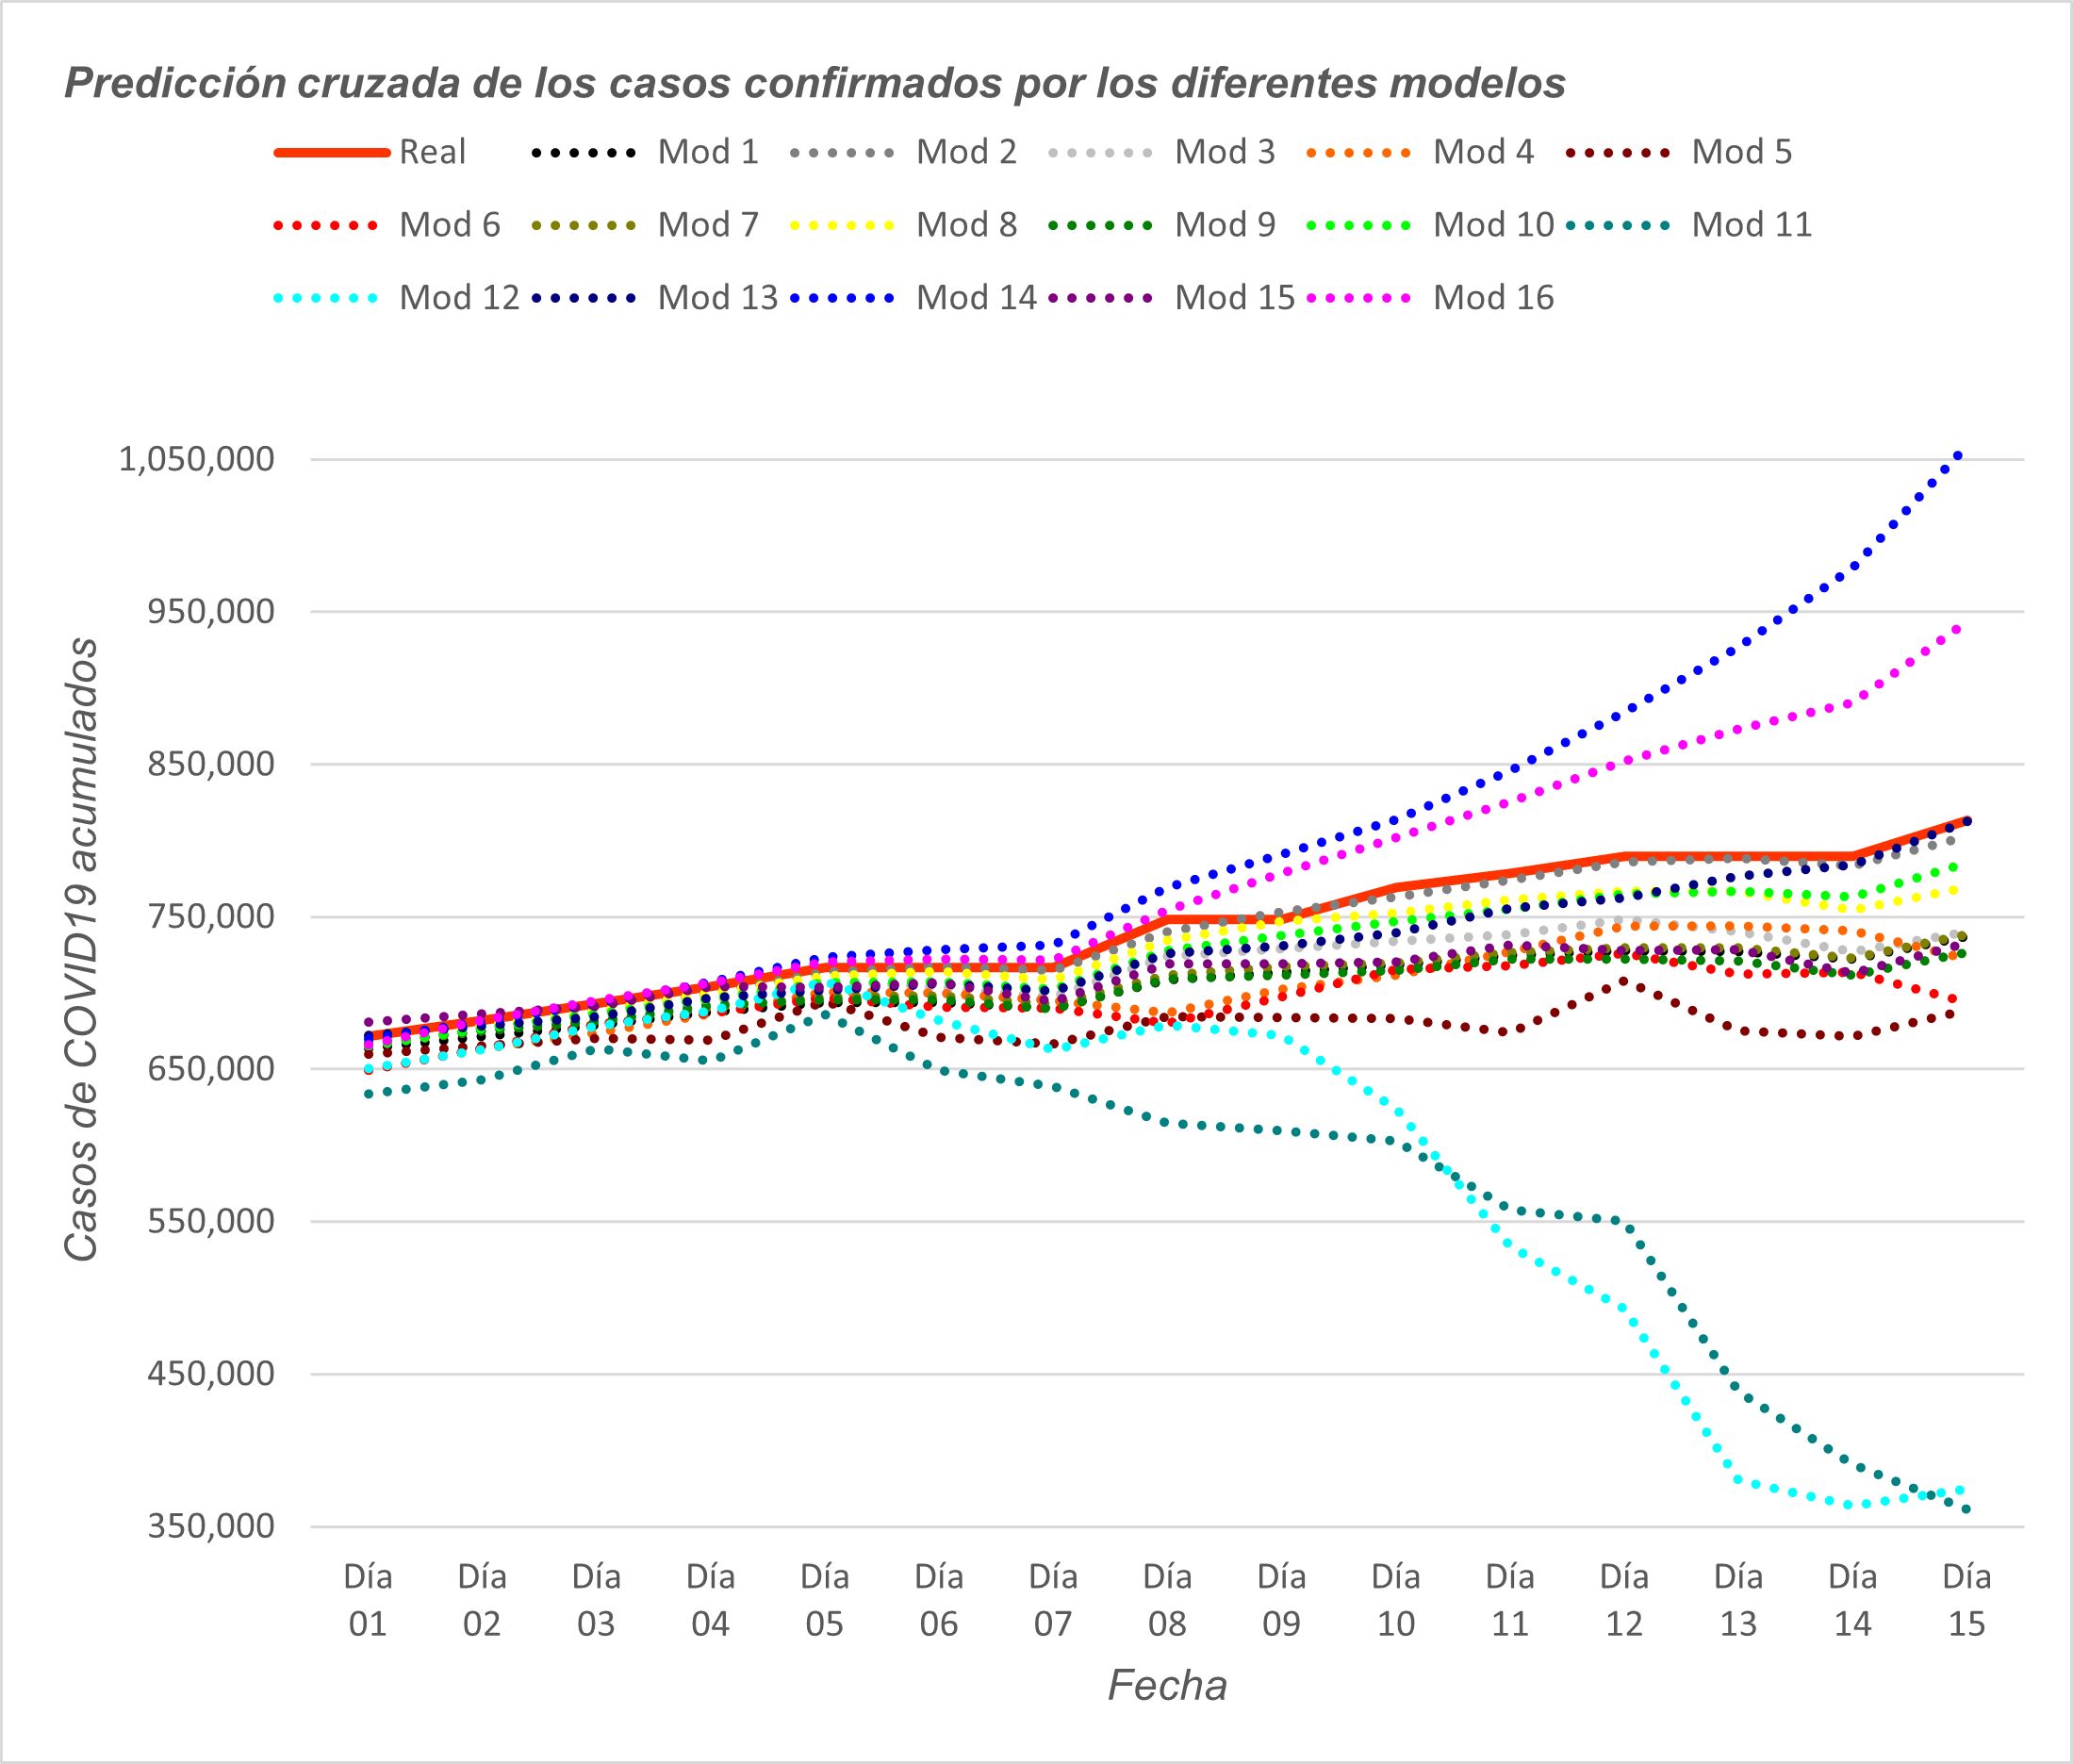
\includegraphics[width=450px]{img/pred_c_conf_ES.png}
            \end{center}

            Seguidamente, se observan los datos de la \textbf{predicción cruzada de casos confirmados}. En comparación con la aislada, aquí parece que casi todos los modelos están bastante cerca de los valores reales hasta el séptimo día, y después, ocurre un poco de todo. \textbf{Algunos se siguen manteniendo muy cerca, como los modelos 2, 8, 10, y 13.} Y por el otro lado, los modelos 14 y 16 empiezan a sobreestimar la cantidad casos rápidamente, mientras que los modelos 12 y 11 los subestiman de una manera ilógica.

            \begin{center}
                \centering
                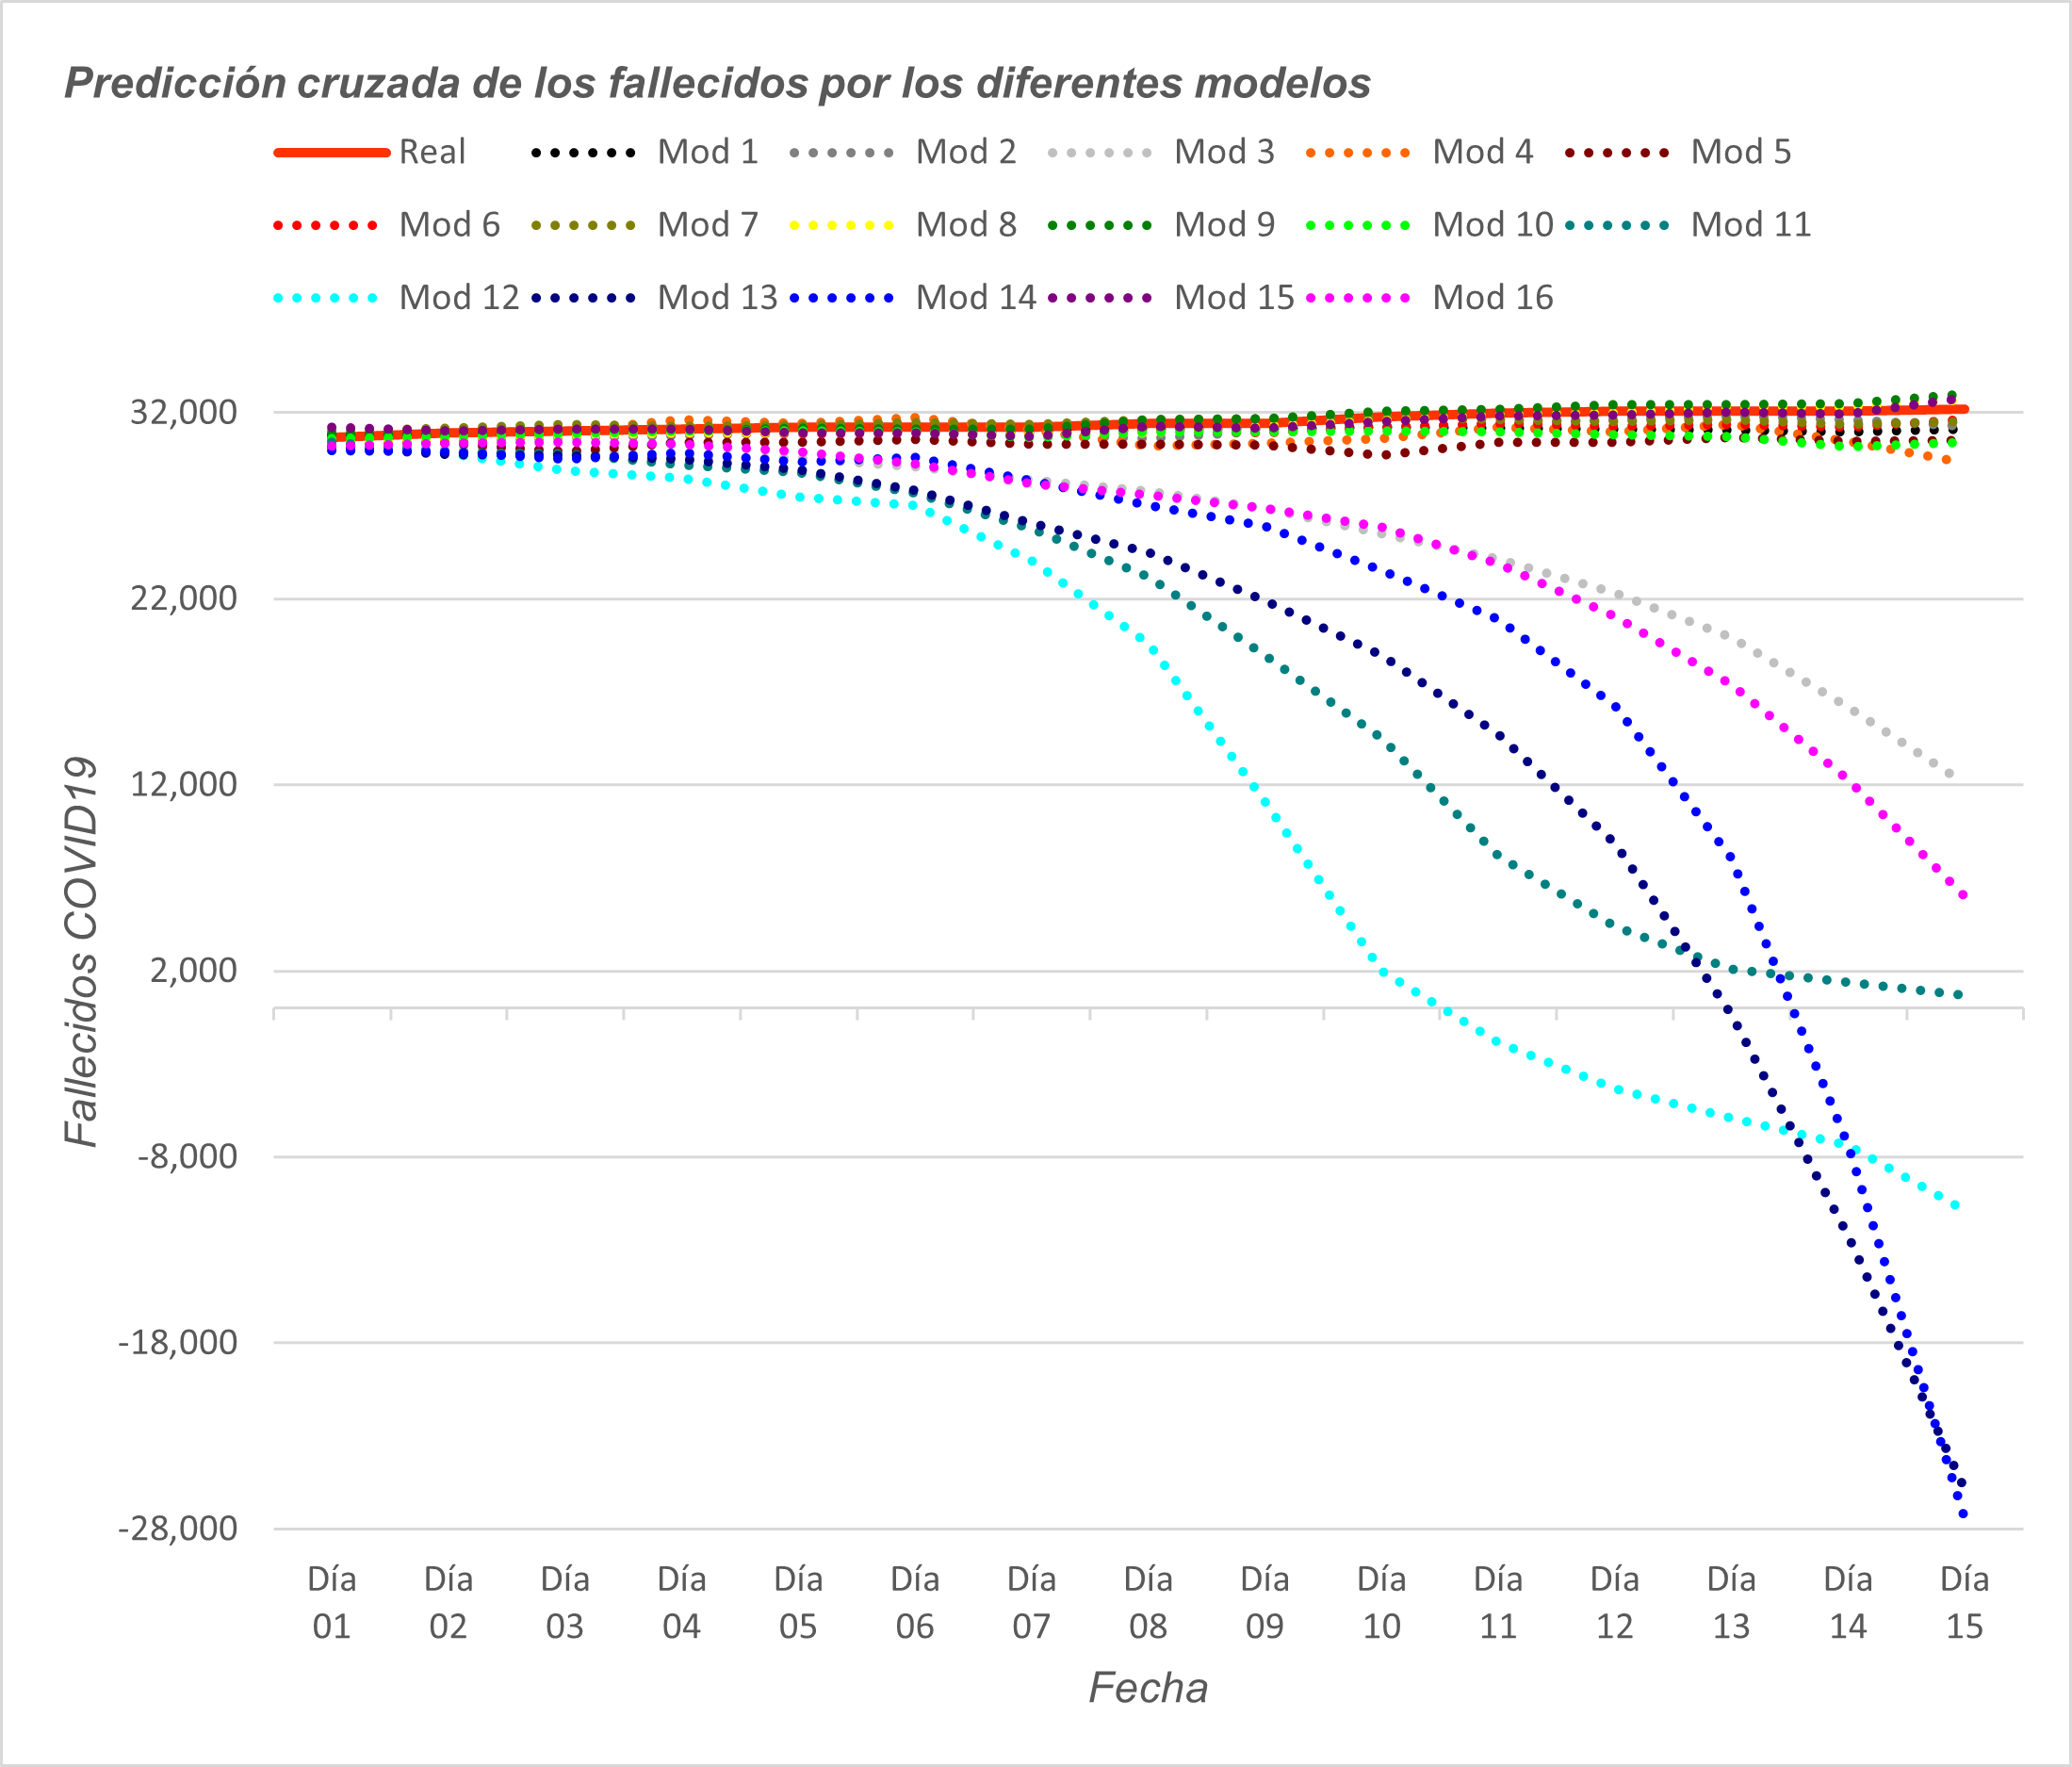
\includegraphics[width=450px]{img/pred_c_fall_ES.png}
            \end{center}

            Para terminar, se tienen las \textbf{predicciones cruzadas de fallecidos}. De manera similar a lo ocurrido en la última gráfica, los modelos en la primera semana parecen coincidir, y una vez empieza la siguiente semana, en este caso, hay seis modelos que indican valores mucho más pequeños, hasta llegar incluso a valores absurdamente negativos. Por otro lado, los otros modelos se acercan bastante bien a los valores reales a simple vista, aunque, hay que tener en cuenta que los valores de fallecidos son más pequeños, así como que la representación de la gráfica es más ajustada, originando todo ello una visión a priori de mejores aproximaciones, aunque sigan difiriendo de los valores reales por bastante.

            \vspace{3mm}

            Una vez visto cada predicción por separado, se va a observar y discutir, en términos de \textbf{errores absolutos}, como se comportan los modelos en general a la hora de predecir todos los casos, tal y como se muestra en la última imagen.

            \begin{center}
                \centering
                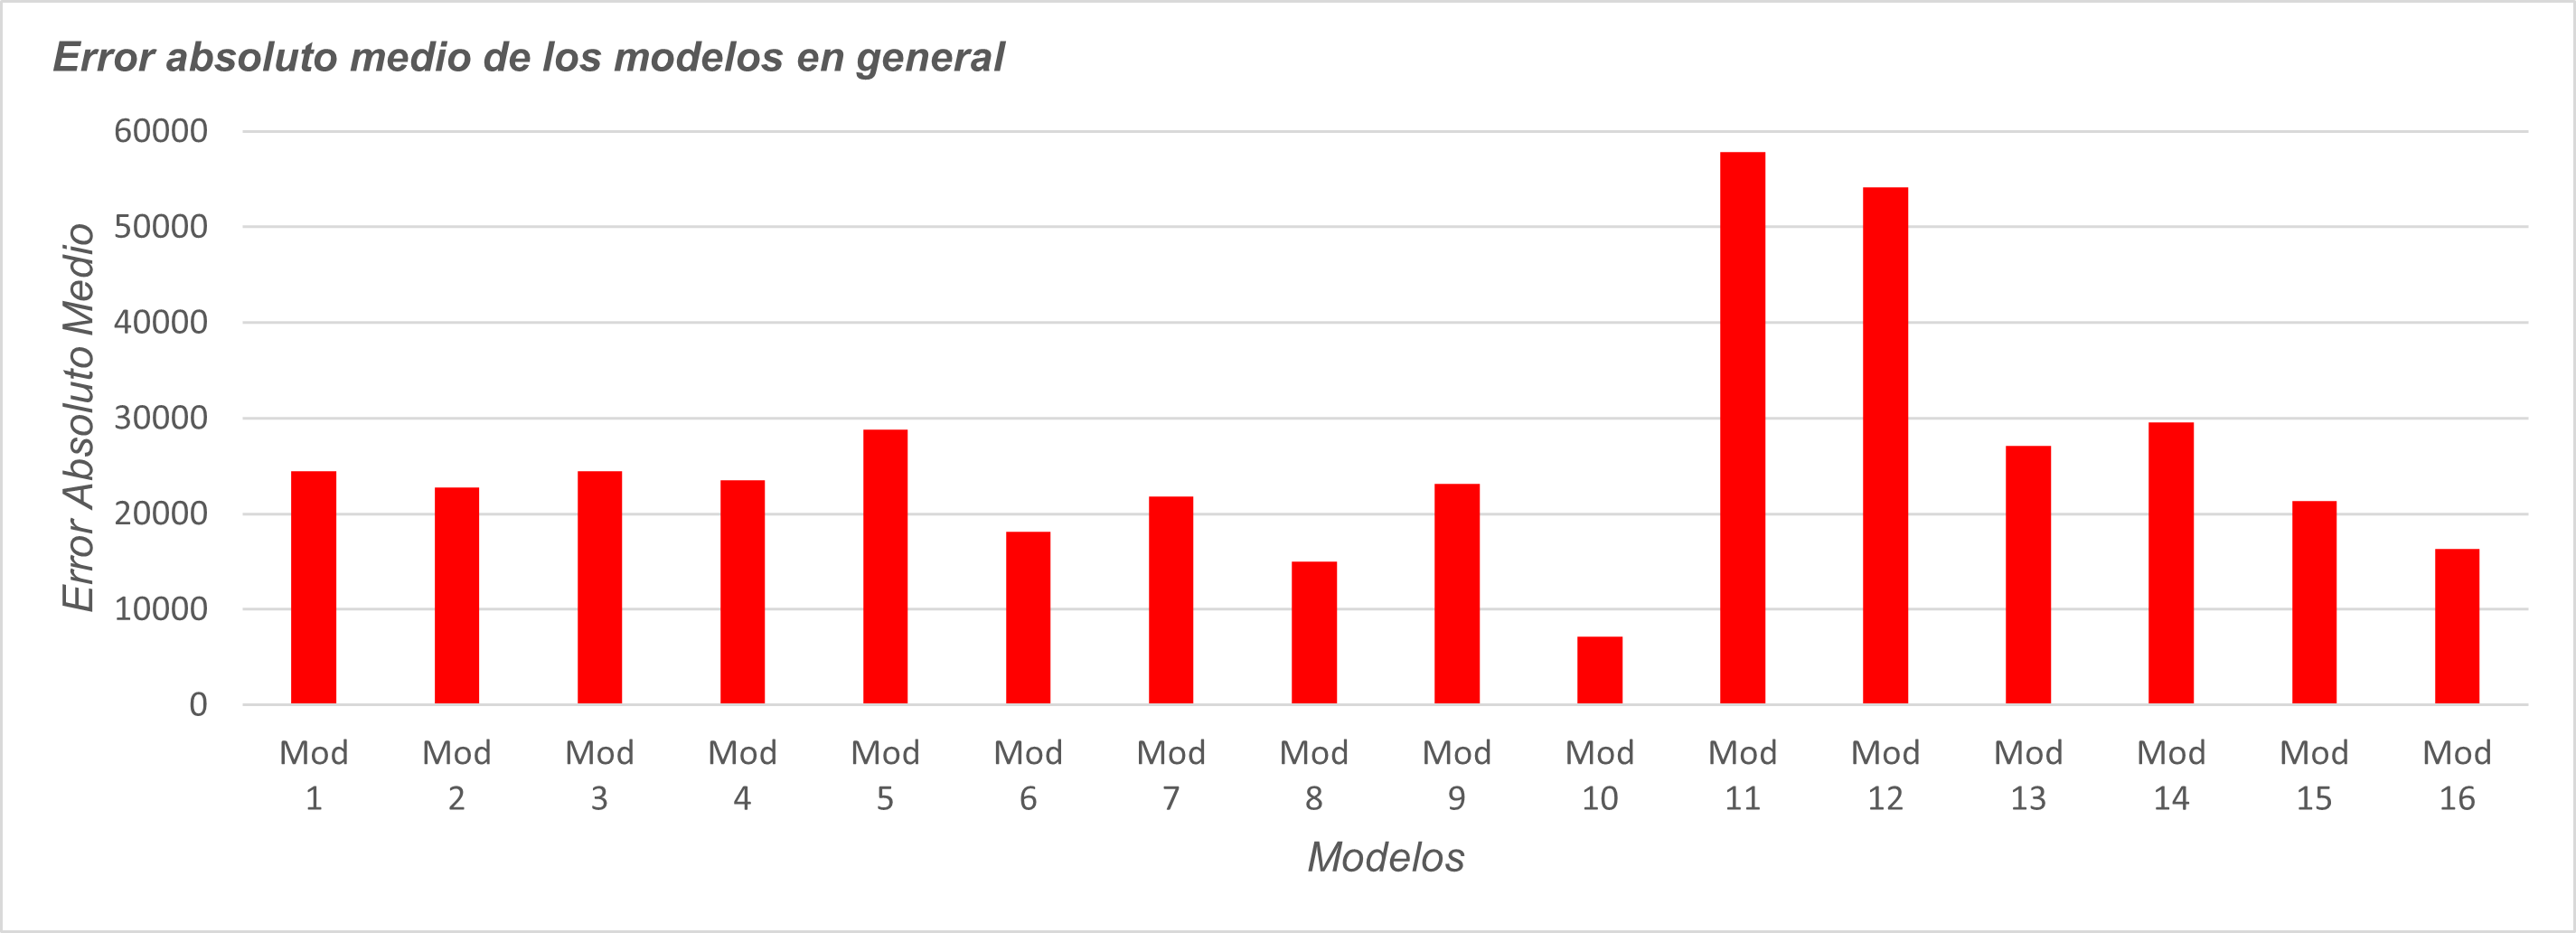
\includegraphics[width=450px]{img/eam_ES_parte2.png}
            \end{center}


            Ya que con las primeras gráficas es complicado ver rápidamente que modelo, de una manera general, aporta predicciones más exactas, con el error absoluto medio de todas las predicciones esto se ve mucho más claro. Como se puede apreciar, el \textbf{modelo 10} es el que ha demostrado ser más regular, obteniendo así el menor error medio, como ya apuntaban las gráficas anteriores. Otros interesantes serían los modelos 6 y 8, que, a pesar de no tener malas cifras, su peor desempeño en la predicción aislada de confirmados hace que su media baje bastante.

            \subsubsection{Resultados de Brasil}

            \begin{center}
                \centering
                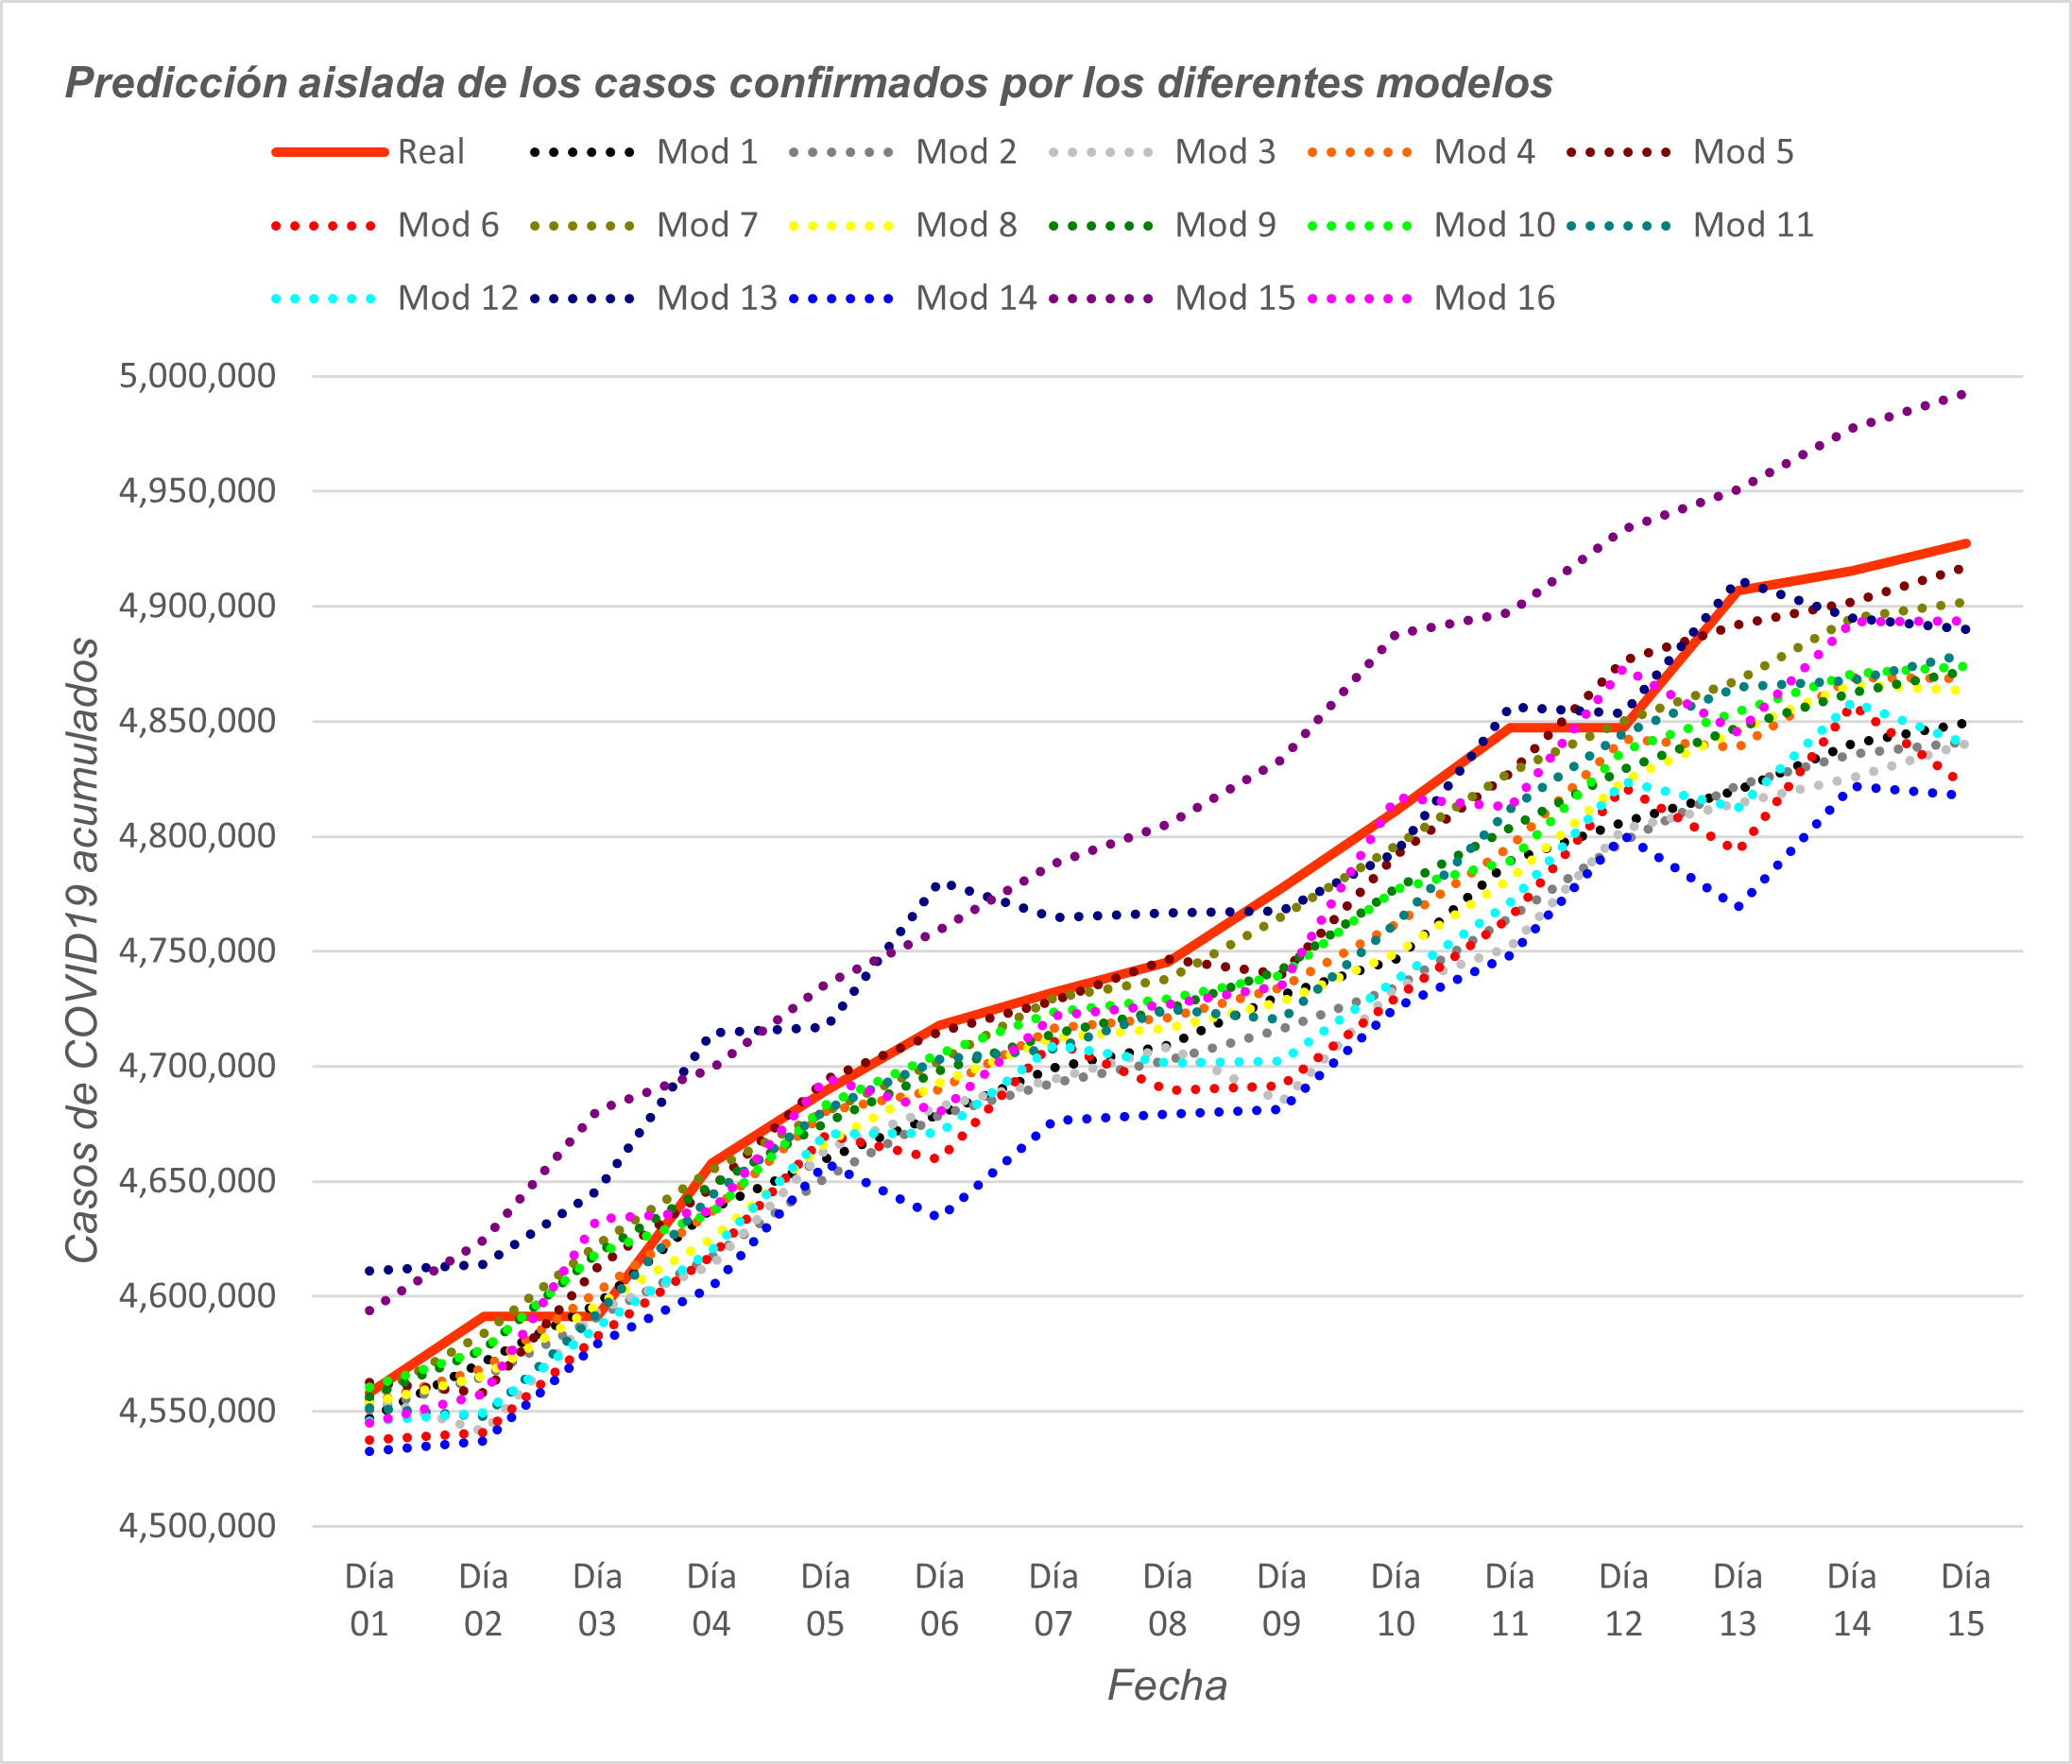
\includegraphics[width=450px]{img/pred_a_conf_BZ.png}
            \end{center}

            De la misma manera, se empieza con la \textbf{predicción aislada de casos confirmados}. Como Brasil presenta valores en los datos muchos más elevados que España, la representación de la gráfica hace que se vean los modelos muchos más parecidos a los datos reales, lo cual no es del todo así. Sin embargo, si que se ve una mejor tendencia que en el caso de España, y aunque se siguen viendo valles donde ocurre un descenso importante de casos, esto ocurre en mucha menor medida.

            \begin{center}
                \centering
                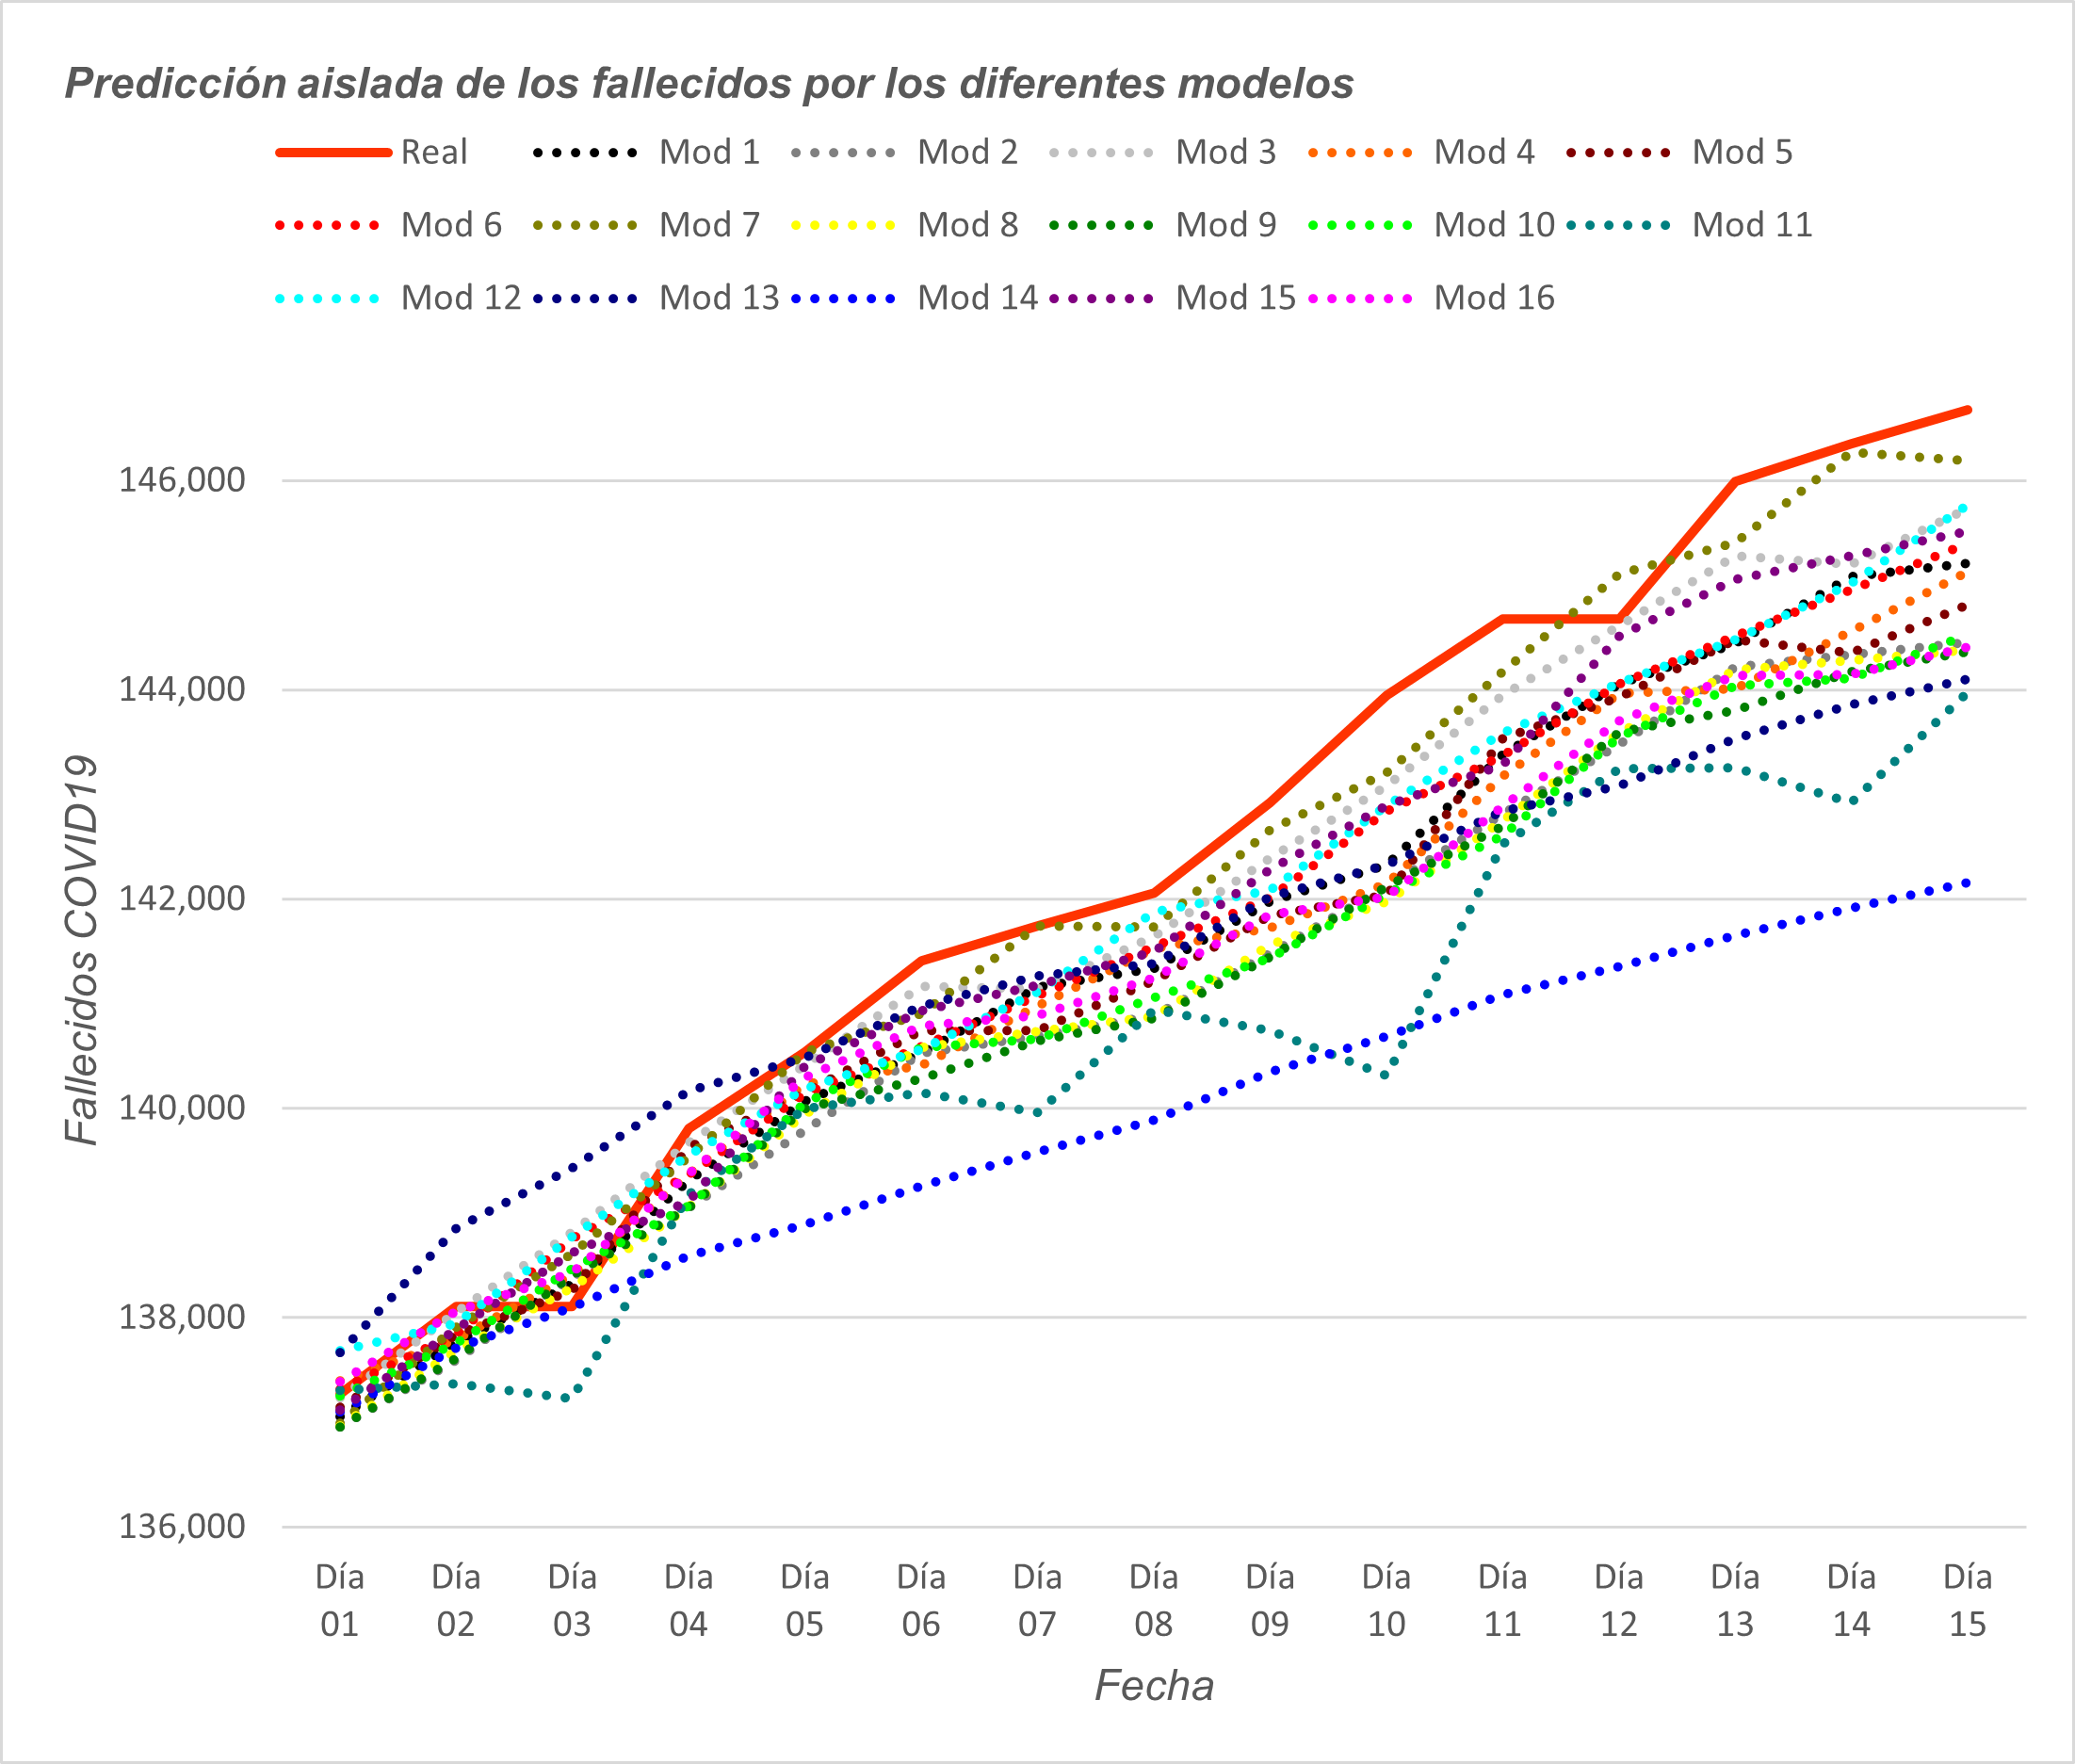
\includegraphics[width=450px]{img/pred_a_fall_BZ.png}
            \end{center}

            La siguiente gráfica corresponde con la \textbf{predicción aislada de fallecidos}, la cual se comporta de manera muy similar a la anterior. Tenemos que, a pesar de encontarse en cifras mucho mayores, el rango entre el que se mueven los modelos es bastante similar, y no están muy alejados de los valores de verdad. Además, la predicción de valores más pequeños ocurre cada vez con menos ocurrencia.

            \begin{center}
                \centering
                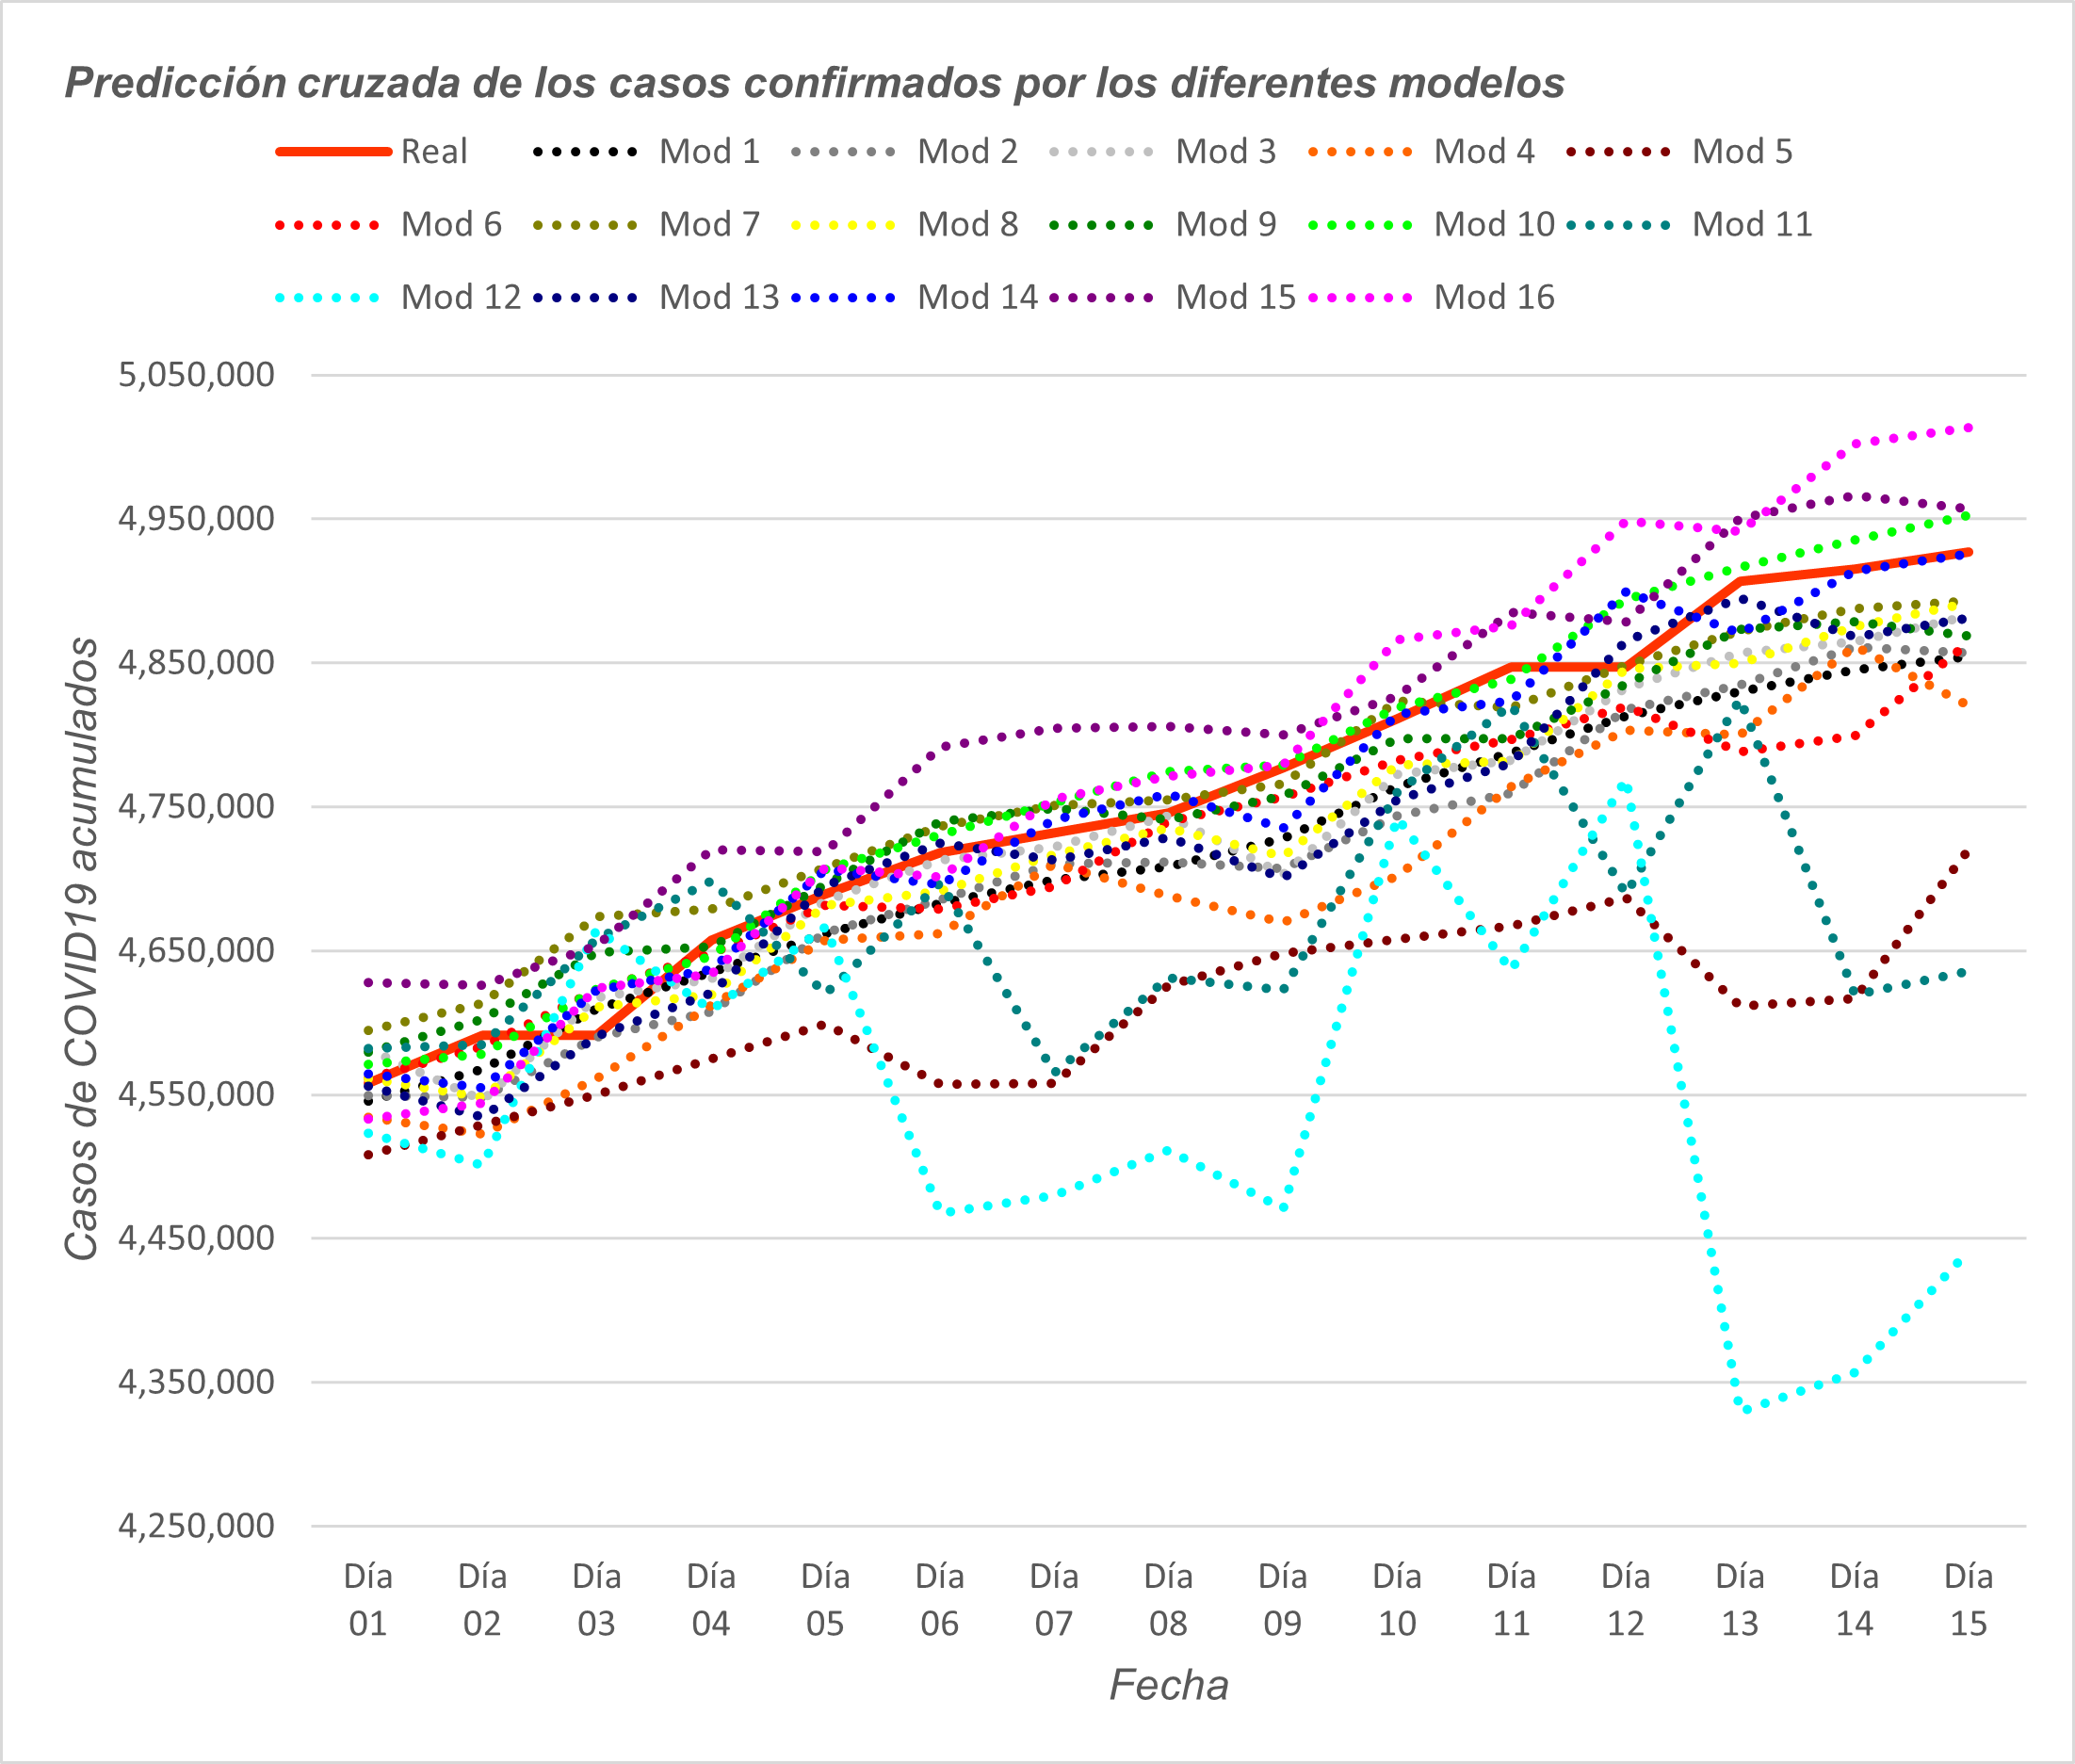
\includegraphics[width=450px]{img/pred_c_conf_BZ.png}
            \end{center}

            Pasamos a la \textbf{predicción cruzada de casos confirmados}, donde encontramos ahora modelos (12 y 11 por ejemplo) que se comportan de una manera más extraña que en los casos anteriores, con picos y valles que no deberían ocurrir dada la naturaleza de los datos. La buena noticia es que una gran parte de los modelos se mueve en torno a los valores reales, y a pesar de ser valores muy elevados, el rango de error tampoco es demasiado grandes de simple vista.

            \begin{center}
                \centering
                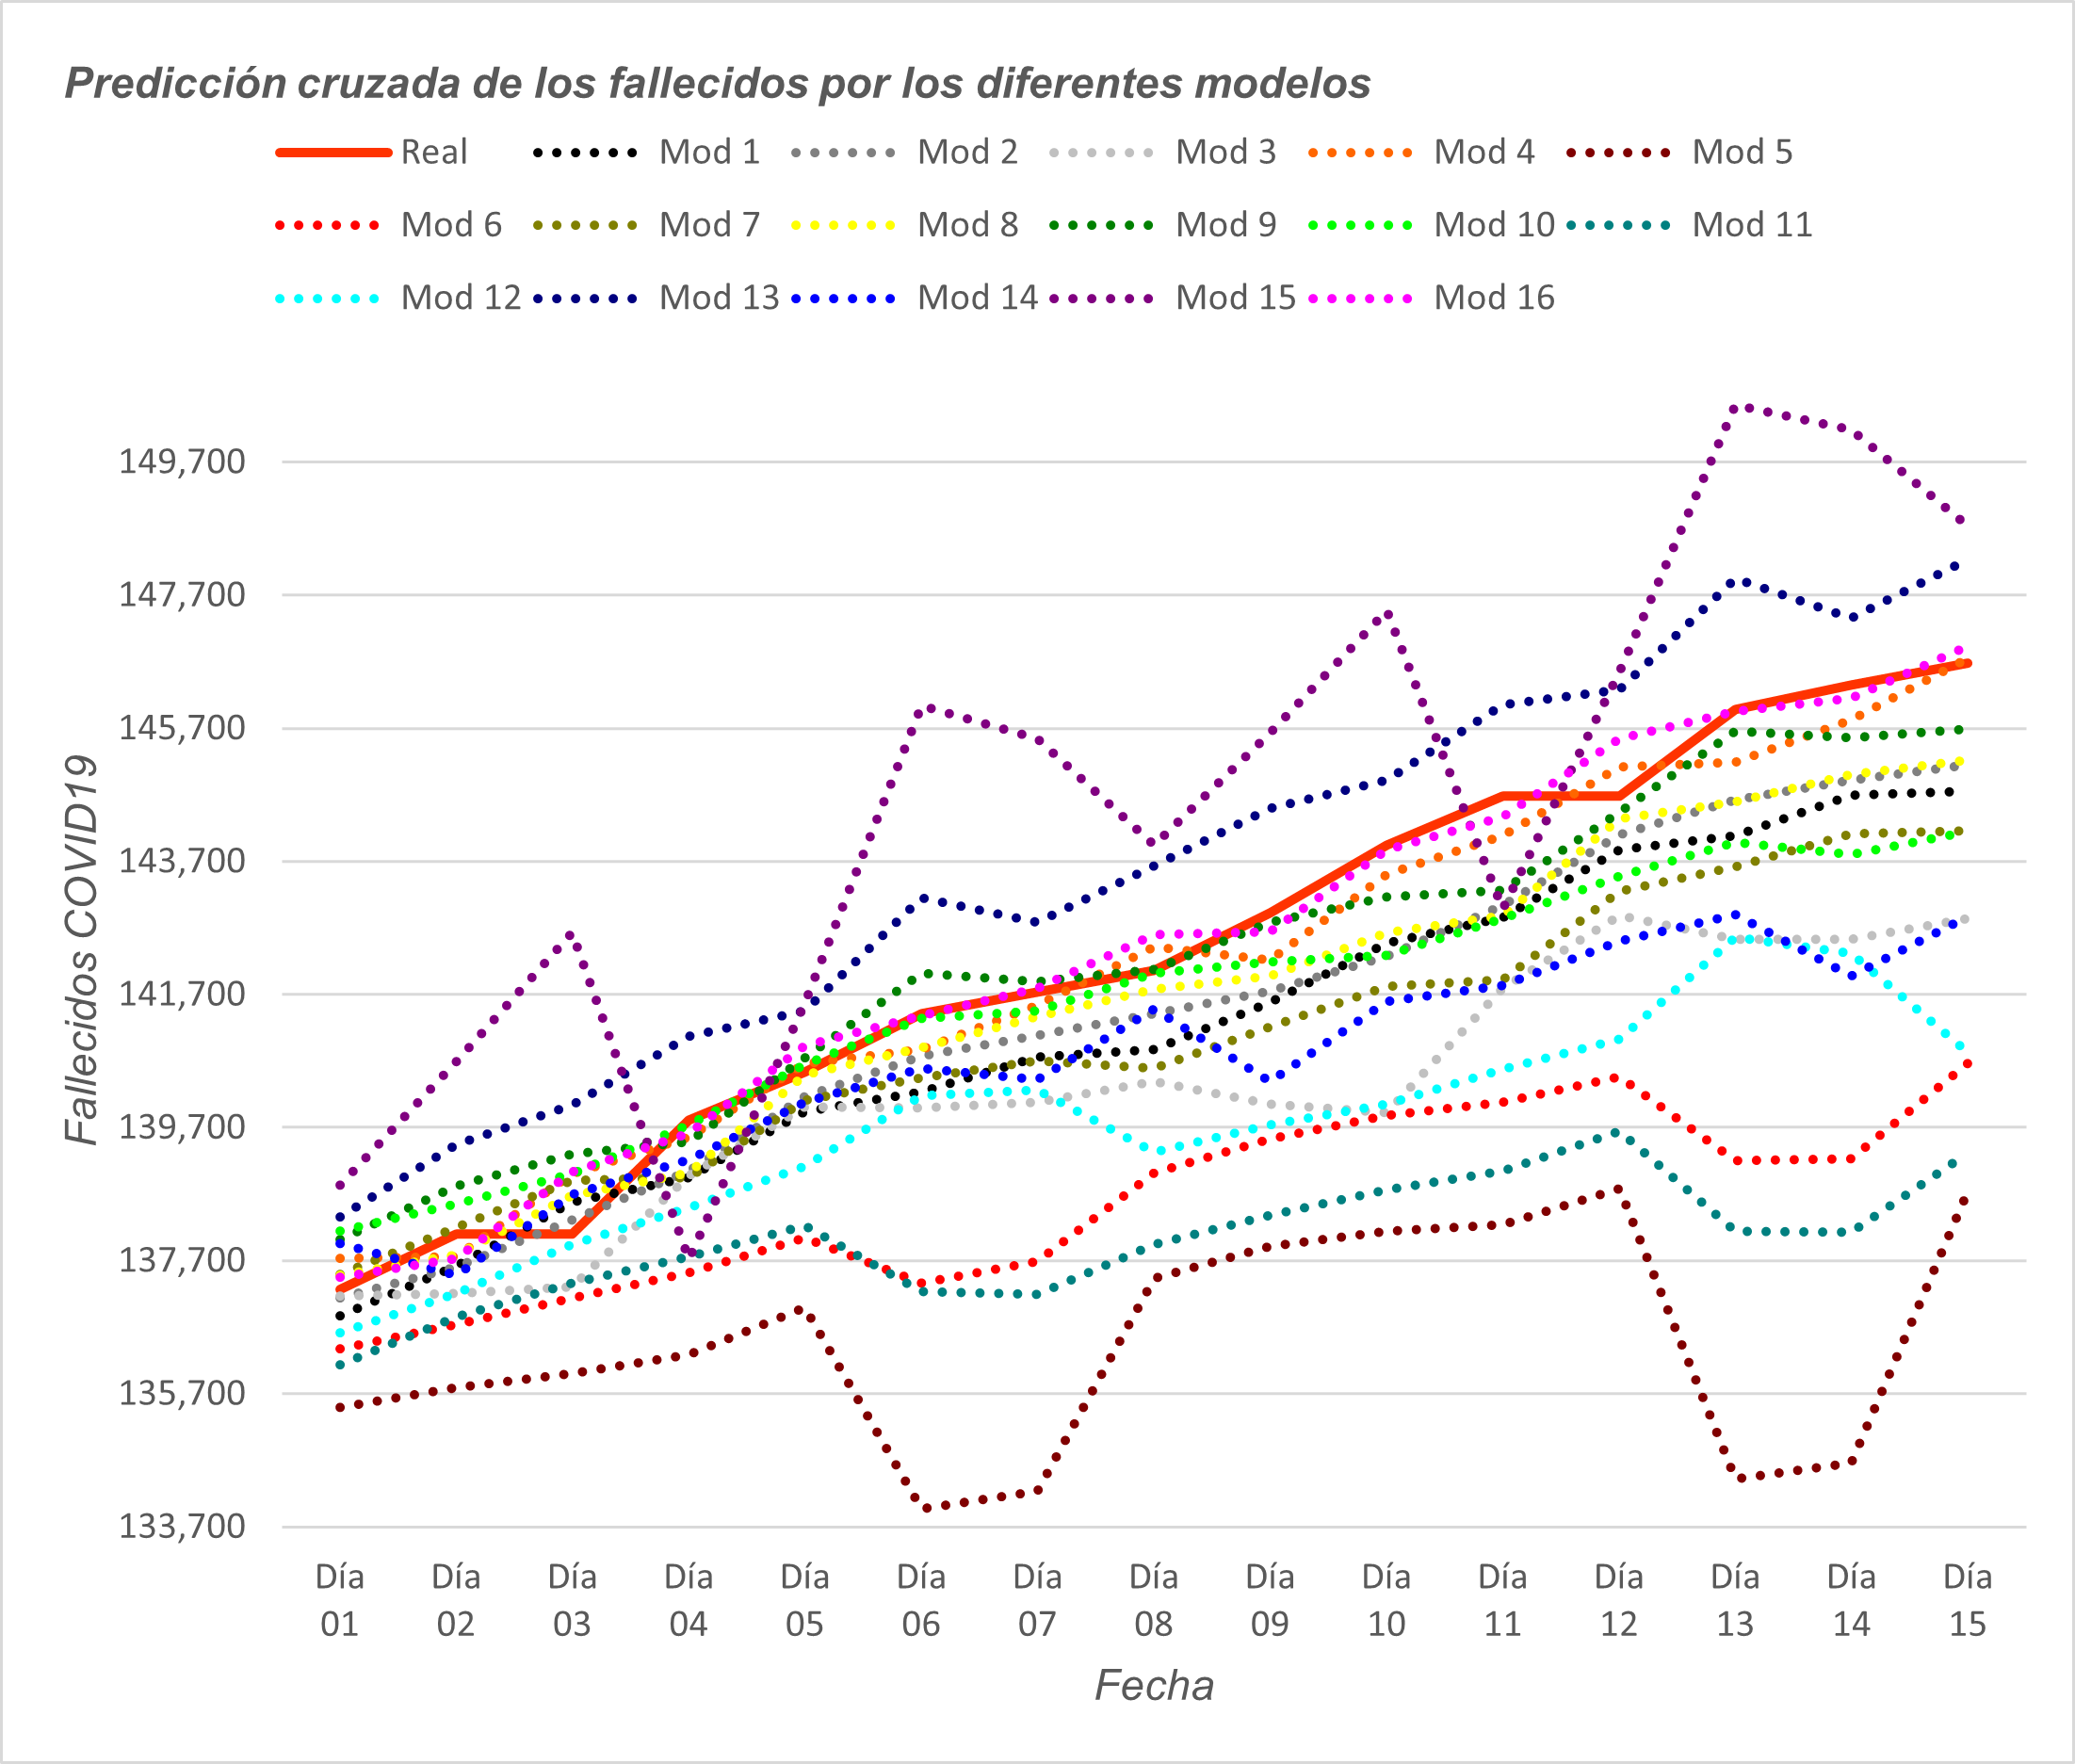
\includegraphics[width=450px]{img/pred_c_fall_BZ.png}
            \end{center}

            Terminamos de nuevo con la \textbf{predicción cruzada de fallecidos}. Como pasaba con la predicción cruzada de confirmados, aumentan los modelos que no generan buenos resultados, e incluso datos que serían imposibles de reproducir. Aquí ya vemos como solo algunos \textbf{modelos como el 16 o el 4 consiguen modelos muy cercanos a los correctos}.

            \newpage

            Ya con el caso de España era complicado dilucidar que modelo o modelos eran mejores a base de las gráficas mostradas, así que ahora con valores muchos más elevados y gráficas más grandes, el uso del \textbf{error absoluto medio} es más necesario que antes.

            \begin{center}
                \centering
                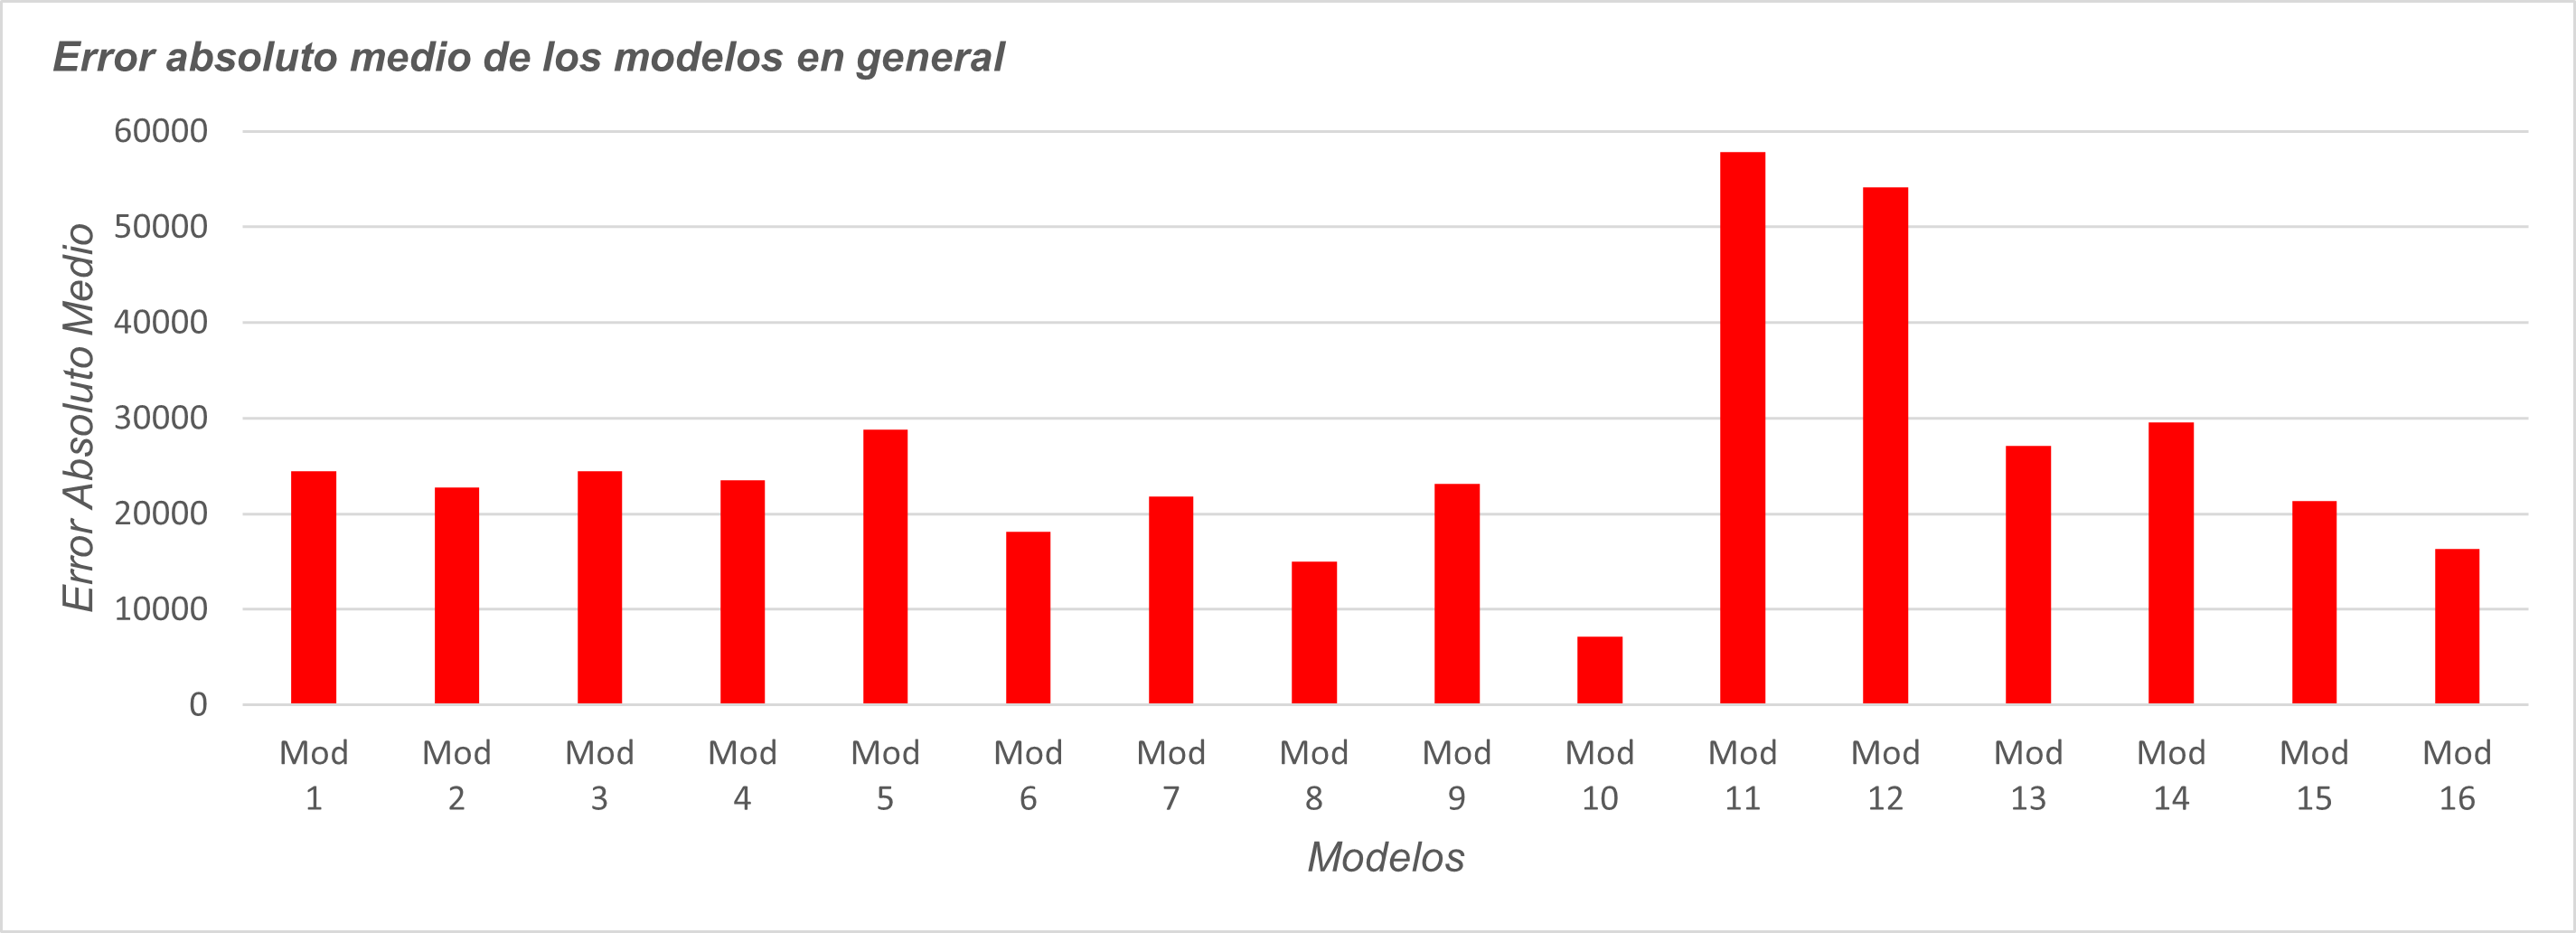
\includegraphics[width=425px]{img/eam_BZ_parte2.png}
            \end{center}

            Se nos demuestra que \textbf{los modelos 7, 9 y 10 son los más regulares}, pues tienen el menor error. De nuevo, es interesante usar este método, pues de otra manera no sería sencillo ver que estos modelos destacan de entre los demás debido a los elevados valores de los datos. También es curioso por el hecho de que no porque un modelo se comporte de manera muy buena en un caso, lo vaya a hacer igual de bien en el resto, como pasa con el modelo 4.

            \vspace{2mm}

            En conclusión, nos encontramos que el \textbf{modelo 10}, que recordamos que es una \textbf{red configurada con 14 días de \textit{lag length}, una capa oculta con ‘a’ neuronas, 0,1 de tasa de aprendizaje y 5000 ciclos}, es el modelo que ha demostrado mejores resultados en ambos países, con errores bastante decentes, así que es el modelo que elegimos. También hay que comentar que en general los modelos con 14 días de \textit{lag length} y 0.1 de razón de aprendizaje funcionan mejor.

            \vspace{2mm}

            \textit{Para ver información más detallada de las gráficas y sus valores, consultar [Anexo 5]}

        \newpage

    \section{Contexto de la práctica}

      La \textit{COVID-19} está asolando al mundo entero. Desde su surgimiento a finales de 2019 se han intentado encontrar diferentes técnicas que sean capaces de frenar su avance. Una de las técnicas con más futuro, y que mejores resultados ha logrado en otros campos similares, es la inteligencia artificial, y, más concretamente, el \textbf{aprendizaje automático}. Tal como comenta \textit{Markus Schmitt} en su artículo del 7 de Abril(nótese su fecha de publicación)[Referencia 5], se pueden usar las diferentes técnicas del aprendizaje automático para resolver los distintos problemas que plantea esta pandemia global, como puede ser \textbf{identificar la población de riesgo}, \textbf{predecir la propagación y origen de la enfermedad} o incluso \textbf{predecir pandemias futuras}, entre otras aplicaciones.

      \vspace{1mm}

      Uno de los principales problemas que se comentan, es la falta de datos necesarios para crear modelos realmente eficaces, ya que su comentario se remonta a los inicios de la pandemia. Pero ahora, 6 meses después, esa cantidad de datos es muchísimo mayor, lo que permite la generación de modelos de aprendizaje automático mucho más robustos y precisos, tal y como se ha mostrado en esta práctica.

      \vspace{4mm}

      Otra de las numerosas maneras en las que la tecnología puede ayudar es la simulación del pliegue de proteínas, esencial para comprender el virus y por tanto la búsqueda de la cura y la vacuna. Uno de los proyectos más interesantes que han surgido al respecto es \textit{folding@home} [Referencia 6], un proyecto de computación distribuida en que están implicados universidades como \textit{Stanford} o la \textit{Universidad de Washington} y empresas como \textit{Google} o \textit{NVIDIA} que buscan simular las dinámicas de las proteínas, incluyendo su pliegue, lo cual explica su nombre.

      \vspace{2mm}

      De manera breve, lo que ellos hacen es usar el poder de cálculo de todos los ordenadores que lo tengan instalado cuando no estén en uso para encontrar la cura de diversas enfermedades como el Coronavirus, pero también el Alzheimer o el Párkinson. Lo único que el usuario debe hacer es seleccionar la cura de la enfermedad a la que desea contribuir y el programa de manera automática aprovechará el tiempo IDLE del ordenador para realizar los cálculos que los científicos necesitan. A continuación se ofrece un  \href{https://www.youtube.com/watch?v=xqvAHnac79U}{\underline{link}} con una pequeña guía de instalación en formato vídeo del software necesario, realizado por uno de los autores de este documento.[Referencia 7]



      \newpage

    \section{Conclusiones}

    Considerando todos los resultados obtenidos a lo largo de este documento, se puede afirmar que las Redes de Neuronas constituyen una buena aproximación a problemas del mundo real como en el caso de la pandemia actual. Los modelos que se generan usando estas técnicas permiten adelantarnos a los sucesos y realizar predicciones con mayor o menor exactitud. Esto es una herramienta muy potente, siempre que se posea de una cantidad de datos lo suficientemente grande.

    \vspace{2mm}

    Sin embargo, se requiere de mucho tiempo de computo para entrenar modelos eficaces y, además, actuan como \textit{cajas negras} y por tanto no tienen la capacidad de explicar sus soluciones. Esto resulta en procesos de prueba y error para encontrar mejores resultados.

    \vspace{2mm}

    En relación con el enfoque de esta práctica, los resultados obtenidos pueden representar la tendencia a seguir de la evolución de la pandemia aunque hay que tener en cuenta que los modelos no son plenamente fiables, entre otras cosas, debido a que los datos tampoco lo son, ya que este tipo de algoritmos se rigen por el principio \textbf{GIGO} (\textit{Garbage In Garbage Out}).

    \vspace{2mm}

    Algunas posibles mejoras para este tipo de modelos sería realizando un estudio previo para los datos, para evitar errores, y conseguir información tomada de forma similar de todas las regiones. De esta forma se evitarían gran cantidad de problemas de los datos. Otra posibilidad para las redes neuronales sería utilizar técnicas de aumento de datos, de forma que se puedan usar más ejemplos distintos durante el entrenamiento.




\clearpage

\section{Referencias}
    \begin{itemize}
        \item [1.] Introduction to Neurons in Neural Networks. Medium. Consultado en Octubre 2020. Url: \\
        \href{https://medium.com/artificial-neural-networks/introduction-to-neurons-in-neural-networks-71828d040a65}{https://medium.com/artificial-neural-networks}
        \item [2.] The complete guide to time series. Consultado en Octobre 2020. Url: \\
        \href{https://towardsdatascience.com/the-complete-guide-to-time-series-analysis-and-forecasting-70d476bfe775}{https://towardsdatascience.com/the-complete-guide-to-time-series}
        \item [3.] COVID Data European Union. Consultado en Octubre 2020. Url: \\
        \href{https://www.ecdc.europa.eu/en/geographical-distribution-2019-ncov-cases}{https://www.ecdc.europa.eu}
        \item [4.] The Humanitarian Data Exchange. Consultado en Octubre 2020. Url: \\
        \href{https://data.humdata.org/dataset/novel-coronavirus-2019-ncov-cases}{https://data.humdata.org/dataset/novel-coronavirus}
        \item [5.] How to fight COVID-19 with machine learning. Consultado en Octubre 2020. Url: \\
        \href{https://towardsdatascience.com/fight-covid-19-with-machine-learning-1d1106192d84}{https://towardsdatascience.com/fight-covid-19-with-machine-learning}
        \item [6.] Folding@home. Consultado en Octubre 2020. Url: \\
        \href{https://foldingathome.org}{https://foldingathome.org}
        \item [7.] Descubre cómo puedes ayudar a encontrar una CURA para el CORONAVIRUS desde tu salón. Consultado en Octubre 2020. Url: \\
        \href{https://www.youtube.com/watch?v=xqvAHnac79U}{https://www.youtube.com/watch?v=xqvAHnac79U}
    \end{itemize}
\printindex



  \section{Anexos}
  \begin{itemize}
    \item [1.] Perceptron Multicapa usando '\textit{K Fold}'\\
    \textbf{\textit{perceptron\_kfold.py}}
    \item [2.] Perceptron Multicapa usando '\textit{split percentage}'\\
    \textbf{\textit{perceptron\_split.py}}
    \item [3.] Programa para realizar la predicción de los modelos\\
    \textbf{\textit{predict.py}}
    \item [4.] Tabla de resultados de los experimentos de la primera parte\\
    \textbf{\textit{valores\_reales\_vs\_predicciones\_\&\_errores\_absolutos\_parte1.xlsx}}
    \item [5.] Tabla de resultados de los experimentos de la segunda parte\\
    \textbf{\textit{valores\_reales\_vs\_predicciones\_\&\_errores\_absolutos\_parte2.xlsx}}
  \end{itemize}


\end{document}
